\documentclass[russian,utf8,emptystyle]{eskdtext}

\usepackage[T2A,T1]{fontenc}

\newcommand{\No}{\textnumero} % костыль для фикса ошибки

\ESKDdepartment{Федеральное государственное бюджетное образовательное учреждение высшего профессионального образования}
\ESKDcompany{Московский государственный технический университет им. Н. Э. Баумана}
\ESKDclassCode{23 0102}
\ESKDtitle{АИС отслеживания и прогнозирования новостных потоков «Волхв»}
\ESKDdocName{Расчетно-пояснительная записка}
\ESKDauthor{Гуща~А.~В.}
\ESKDtitleApprovedBy{~}{~\underline{\hspace{2.5cm}}}
\ESKDtitleAgreedBy{~}{~\underline{\hspace{2.5cm}}}
\ESKDtitleDesignedBy{Студент группы ИУ5-122}{Гуща~А.~В}

\usepackage{multirow}
\usepackage{tabularx}
\usepackage{tabularx,ragged2e}
\usepackage{pdfpages}
\renewcommand\tabularxcolumn[1]{>{\Centering}p{#1}}
\newcommand\abs[1]{\left|#1\right|}

\usepackage{longtable,tabu}

\usepackage{geometry}
\geometry{footskip = 1cm}

\pagenumbering{arabic}
\pagestyle{plain}

\usepackage{setspace}

\usepackage{xcolor}
\usepackage{listings}
\lstset{
    breaklines=true,
    postbreak=\raisebox{0ex}[0ex][0ex]{\ensuremath{\color{red}\hookrightarrow\space}},
    extendedchars=\true,
    basicstyle=\small,
    inputencoding=utf8,
    numbers=left,                    
    numbersep=5pt,                  
    numberstyle=\tiny\color{mygray},
}
\renewcommand{\lstlistingname}{Листинг}
\renewcommand{\lstlistlistingname}{Листинги}

\ESKDsectAlign{section}{Center} % to capitalize russian text

\usepackage{array}
\newcolumntype{L}[1]{>{\raggedright\let\newline\\\arraybackslash\hspace{0pt}}m{#1}}
\newcolumntype{C}[1]{>{\centering\let\newline\\\arraybackslash\hspace{0pt}}m{#1}}
\newcolumntype{R}[1]{>{\raggedleft\let\newline\\\arraybackslash\hspace{0pt}}m{#1}}

\usepackage{tikz}
\usepackage{pgf-pie}

\usepackage{totcount}
\regtotcounter{figure}
\regtotcounter{table}

%\usepackage{titlesec}
\usepackage{hyperref}

\setcounter{secnumdepth}{5}
\setcounter{tocdepth}{5}

%\renewcommand*{\thesection}{\arabic{section}}

%===========================================================================
\begin{document}

\clearpage
\clearpage

\pagenumbering{gobble}
\section*{Реферат}
%\pageref{LastPage}
Данная расчетно-пояснительная записка содержит 156 (без приложения) страниц, \total{figure} иллюстраций (без приложения), \total{table} таблиц, 3 приложения, 24 использованных источников.

Ключевые слова: полнотекстовый поиск, сбор информации, формальный язык запросов, генетическое программирование, эволюционные алгоритмы, символьная регрессия, прогноз временных рядов.

Данный дипломный проект посвящен разработке автоматизированной информационной системы для анализа новостных потоков, а также прогнозирования их активности. Целью разработки является сбор информации из открытых источников, накопление данной информации в СУБД, проведение анализа накопленных новостных данных на основе проблемно ориентированного языка программирования и предсказание количества новостей по определенной тематике с помощью эволюционных методов прогнозирования.

Система проектируется в виде веб-сервиса, предоставляющих пользователю набор экранных форм для взаимодействия с данным программных изделием, а также машинный интерфейс для взаимодействия стороннего программного обеспечения с данной АИС. Структуру системы составляют сервер приложения, сервер СУБД, сервер индексации и терминалы пользователей. При разработке программного продукта используется язык программирования Haskell.

В результате разработки была спроектирована автоматизированная информационная система, отвечающая требованиям технического задания и имеющая возможности, необходимые как для сбора и хранения новостной информации в базах данных, так и для всестороннего ее анализа.

Область применения АИС -- лаборатории анализа данных, составной компонент в распределённых системах анализа данных. Проект является некоммерческим с малой стоимостью выполнения.


\tableofcontents

\include{normReferences}
\section*{Определения, обозначения и сокращения}

\begin{itemize}
\item АИС -- автоматизированная информационная система.
\item АПК -- аппаратно-программный комплекс.
\item БД -- база данных.
\item ЕСКД -- единая система конструкторской документации.
\item Управляющий класс (control) -- класс модели анализа, представляющий координацию, последовательность и управление другими объектами, часто используется для инкапсуляции управления для варианта использования.
\item Граничный класс (boundary) -- класс модели анализа, используемый для моделирования взаимодействия между системой и ее актантами, то есть пользователями и внешними системами.
\item Класс сущности (entity) -- класс модели анализа, используемый для моделирования долгоживущей, часто персистентной информации.
\item ОЗУ -- оперативное запоминающее устройство.
\item ОС -- операционная система.
\item ПК -- персональный компьютер.
\item ПО -- программное обеспечение.
\item ПЭВМ -- персональная электронно-вычислительная машина.
\item СанПиН -- санитарно-эпидемиологические правила и нормативы.
\item СИБИД -- система стандартов по информации, библиотечному и издательскому делу.
\item СНиП -- строительные нормы и правила. 
\item ССБТ -- система стандартов по информации, библиотечному и издательскому делу.
\item СУБД -- система управления базами данных.
\item ЭВМ -- электронно-вычислительная машина.
\item ЭМП -- электромагнитное поле.
\item API -- application programming interface -- набор готовых классов, процедур, функций, структур и констант, предоставляемых приложением (библиотекой, сервисом) для использования во внешних программных продуктах.
\item CPU -- central processing unit -- центральный процессор.
\item HDD -- hard disk drive -- жесткий диск.
\item SQL -- structured query language -- универсальный компьютерный язык, применяемый для создания, модификации и управления данными в реляционных базах данных. SQL основывается на исчислении кортежей. SQL является, прежде всего, информационно-логическим языком, предназначенным для описания, изменения и извлечения данных, хранимых в реляционных базах данных. 
\item UML -- unified modeling language, унифицированный язык моделирования -- язык графического описания для объектного моделирования в области разработки программного обеспечения. UML является языком широкого профиля, это открытый стандарт, использующий графические обозначения для создания абстрактной модели системы, называемой UML-моделью.
\item GUI -- graphical user interface, графический интерфейс пользователя -- разновидность пользовательского интерфейса, в котором элементы интерфейса (меню, кнопки, значки, списки и т. п.), представленные пользователю на дисплее, исполнены в виде графических изображений.
\item FRP -- functional reactive programming, функциональное реактивное программирование -- парадигма программирования на основе функциональной парадигмы, используемая для разработки GUI, роботостроения и генерации музыки с помощью явного управлением модельным временем.
\item ЛВС -- локальная вычислительная сеть.

\end{itemize}
\include{introduction}

%===========================================================================
% Конструкторская часть
\section{Технологическая часть}

\subsection{Общее описание программного комплекса}
\subsubsection{Функциональное назначение}

Разработанная АИС предназначена для автоматизации перечисленных процессов:
\begin{itemize}
\item Ввод документа в систему;
\item Построение ускоряющего поиск индекса;
\item Выполнение полнотекстового поиска на основе формализованного языка запросов;
\item Просмотр документов и их редактирование;
\item Выполнение операций над индексом;
\item Рубрикация документов и сохранённых запросов;
\item Прогнозирование новостных потоков.
\end{itemize}

Разработанная АИС должна работать в режиме веб-приложения, в соответствии с выбранной на этапе проектирования архитектурой. Процесс развертывания системы не должен быть чрезмерно сложен или требовать нереалистичных объемов времени.

\subsubsection{Средства технического обеспечения}

Для корректного функционирования программного комплекса необходимы следующие технические средства, имеющие характеристики не меньше указанных.

\paragraph*{Сервер} \hfill

Персональная ЭВМ архитектуры AMD x86\_64:
\begin{itemize}
\item процессор Intel i7-860 (4 ядра, 2.8 ГГц);
\item жесткий диск не менее 1 Тб;
\item оперативная память 4 Гб;
\item сетевой адаптер для подключения к ЛВС.
\end{itemize}

\paragraph*{Сервер индексации} \hfill

Персональная ЭВМ архитектуры AMD x86\_64:
\begin{itemize}
\item процессор Intel i7-860 (4 ядра, 2.8 ГГц);
\item жесткий диск не менее 500 Гб;
\item оперативная память 8 Гб;
\item сетевой адаптер для подключения к ЛВС.
\end{itemize}

\paragraph*{Клиентская машина} \hfill

Персональная ЭВМ архитектуры AMD x86\_64 или IBM x86:
\begin{itemize}
\item процессор Intel Pentium Dual-Core;
\item жесткий диск не менее 100 Гб;
\item оперативная память 2 Гб;
\item сетевой адаптер для подключения к ЛВС.
\item Клавиатура, мышь, экран;
\end{itemize}


\subsubsection{Программное обеспечение, необходимое для функционирования}

Для функционирования АИС требуется следующее ПО.

  \paragraph*{Серверное ПО} \hfill

  \begin{itemize}
  \item Astra Linux 1.4 релиз <<Смоленск>>;
  \item СУБД PostgreSQL версии 9.4;
  \item Библиотека gmp версии 3 для работы с целочисленными числами произвольной точности;
  \item Библиотека pcre версии 3 для работы с регулярными выражениями;
  \item Клиентская библиотека от MySQL для протокола связи между сервером приложения и сервером индексации;
  \item Библиотека expat для работы с XML файлами;
  \end{itemize}

  \paragraph*{Клиентское ПО} \hfill

  \begin{itemize}
  \item Любая ОС;
  \item Браузер Firefox версии 46 или Chrome версии 51;
  \end{itemize}

\subsection{Структура программы с описанием функций составных частей}

Разрабатываемая АИС запаковывается в пакеты формата \textbf{deb}. Система поставляется в трех пакетах:
\begin{itemize}
\item volchv-ips-server -- сервер приложений АИС.
\item volchv-ips-indexer -- сервер индексации АИС.
\item volchv-predictor -- сервис прогнозирования АИС.
\end{itemize}

\subsubsection{Архив сервера приложений}  \hfill

Архив сервера приложений состоит из:
\begin{itemize}
\item \textbf{etc/init.d/volchv-ips-server} -- конфигурационный файл сервиса ОС для сервера приложений. 
\item \textbf{etc/volchv/ips-server.yml} -- конфигурационный файл сервера приложений.
\item \textbf{usr/bin/ips} -- исполняемый файл сервера приложений, который устанавливается как сервис ОС. 
\item \textbf{var/lib/volchv/ips-server/static} -- статичные файлы сервера приложений, содержащие HTML, CSS и JavaScript файлы клиентской части АИС.
\end{itemize}

\subsubsection{Архив сервера индексации} \hfill

Архив сервера индексации состоит из:
\begin{itemize}
\item \textbf{etc/init.d/volchv-ips-indexer} -- конфигурационный файл сервиса ОС для сервера индексации. 
\item \textbf{etc/volchv/ips-indexer} -- конфигурационные файлы и словари русского и английского языков.
\item \textbf{usr/bin} -- исполняемые файлы сервера индексации, необходимые для разбора слов, поиска по словарям, отладки и обработки формализованныйх запросов. 
\item \textbf{usr/share} -- файлы документации для внутренних инструментов отладки сервера индексации.
\end{itemize}

\subsubsection{Архив сервиса прогнозирования} \hfill

Архив сервиса прогнозирования состоит из:
\begin{itemize}
\item \textbf{etc/init.d/volchv-predictor} -- конфигурационный файл сервиса ОС для сервиса прогнозирования. 
\item \textbf{etc/volchv/predictor.yml} -- конфигурационный файл сервиса прогнозирования.
\item \textbf{usr/bin/predictor} -- исполняемый файл сервера приложений, который устанавливается как сервис ОС. 
\item \textbf{var/lib/volchv/predictor/static} -- статичные файлы сервиса прогнозирования, содержащие HTML, CSS и JavaScript файлы дополнительной клиентской части АИС для поддержки функций прогнозирования.
\end{itemize}

\subsection{Установка и запуск приложения}

Для установки АИС следует провести следующие действия:
\begin{enumerate}
\item Установить все необходимое ПО на серверах для сервера приложений и сервера индексирования.
\item Выполнить подключение репозиториев с пакетами Astra Linux согласно руководству системного администратора Astra Linux.
\item С помощью программы \textbf{dpkg} и \textbf{apt-get} произвести установку пакетов АИС. Установка производится согласно руководству системного администратора Astra Linux.
\item В конфигурационных файлах, перечисленных выше, сервера приложений и сервера индексации указать взаимные адреса серверов.
\item Проверить работоспособность системы и приступить к её эксплуатации.
\end{enumerate}

\subsection{Внутренне проектирование}
\subsubsection{Разработка структуры системы}

Разрабатываемая система является самостоятельным продуктом, но следует помнить о полезности модульного подхода для возможности расширения и модернизации. Архитектура системы отражены в графической части дипломного проекта на листе «Структурная схема».

\paragraph{Анализ информационных потоков} \hfill

Анализ информационных потоков выявил следующие источники и потребителей информации:
\begin{itemize}
\item Пользователь -- является одновременно и потребителем и источником информации. Пользователь создает формализованные запросы и определяет настройки системы, а потребляет данные, обработанные АИС;
\item Новостные сайты -- источники информации, с которых производится сбор сообщений;
\end{itemize}

\paragraph{Определение состава компонентов системы} \hfill

Согласно требованиям ТЗ касательно функциональности разрабатываемого комплекса, можно выделить следующие составляющие компоненты.

\subparagraph{Модуль рубрикатора новостей и сохранённых запросов.} \hfill

Должен предоставлять пользователю интерфейс для просмотра и редактирования рубрик (категорий) новостей, а также сохранение, редактирование и удаление сохранённых запросов, которые привязываются к рубрикам. Рубрики должны образовывать древовидную структуру, листами которой являются либо рубрики, либо сохранённые запросы. Для каждой рубрики должно отображаться количество новостей, относящихся к данной рубрике. Отсутствие рубрики у сохранённого запроса или у новости должно обрабатываться и отображаться пользователю как специальная рубрика «Нерубрицированные».

Входные данные:
\begin{itemize}
\item Действия над рубриками и запросами: добавление, удаление, обновление;
\item Данные рубрик: название и положение в дереве из рубрик;
\item Данные сохранённых запросов: тело запроса на \\ проблемно-ориентированном языке, дополнительные фильтры на дату публикации, источник и теги документаю
\end{itemize}

Выходные данные:
\begin{itemize}
\item Рубрикатор с рубриками и количеством документов в них;
\item Сохранённые запросы, прикреплённые к рубрикам;
\end{itemize}

\subparagraph{Модуль поиска новостей и формализованных запросов.}  \hfill

Должен предоставлять пользователю интерфейс для ввода поискового запроса на
естественном языке или на формализованном языке запросов. Поиск должен
иметь возможность:
\begin{itemize}
\item настройки сортировки по времени новости и её релевантности запросу;
\item указания интервала времени для поиска;
\item дополнительной фильтрации по реквизитам документа;
\item поиска с условием наличия/отсутствия конкретных меток новостей.
\end{itemize}

Формализованные поисковые запросы должны иметь возможность:
\begin{itemize}
\item Поиска с учётом морфологии Русского и Английского языков;
\item Поиска с учётом максимального расстояния между ключевыми словами;
\item Поиска фиксированной фразы;
\item Поиска по конкретному реквизиту документа;
\item Поиска по ключевым словам, расположенных в конце и начале реквизита;
\item Поиска по ключевым словам с указанием приоритета для каждого из них;
\item Поиска в пределах одного предложения или параграфа;
\item Поиска с составными запросами, части которого объединены логическим оператором «ИЛИ».
\end{itemize}

Входные данные:
\begin{itemize}
\item Запрос на проблемно-ориентированном языке.
\end{itemize}

Выходные данные:
\begin{itemize}
\item Список документов, удовлетворяющих запросу. Текст документа должен содержать разметку, указывающую на части текста, которые соответствуют запросу.
\item Количество документов, всего удовлетворяющих запросу.
\item Время выполнения запроса.
\end{itemize}

\subparagraph{Модуль просмотра новости.} \hfill

Должен предоставлять пользователю полную информацию о документе (новости) и его реквизитах. Также модуль должен предоставлять возможность редактировать реквизиты документа (за исключением идентификатора и источника) и возможность удаления новости из АИС.

Реквизиты документа:
\begin{itemize}
\item Заголовок новости -- краткий заголовок новости;
\item Основная часть новости -- основной массив текста с форматированием;
\item Время публикации новости -- время публикации новости, указанное в
источнике;
\item Рубрика новости -- категория новости, к которой она относится;
\item Источник новости -- адрес сайта новости;
\item Идентификатор новости -- уникальный идентификатор новости, под
которым она хранится в БД.
\item Метки новости -- список строк-меток, которые были присвоены новости;
\end{itemize}

Входные данные:
\begin{itemize}
\item Запрос на проблемно-ориентированном языке для подсветки основной части документа. Может отсутствовать, тогда отображается весь текст документа без подсветки.
\item Идентификатор документа для отображения.
\item Обновленные значения реквизитов документа при их редактировании.
\end{itemize}

Выходные данные:
\begin{itemize}
\item Реквизиты документа, перечисленные выше.
\item Обновлённые данные в базе данных и индексе при редактировании полей документа.
\end{itemize}

\subparagraph{Модуль управления индексом.} \hfill

Должен предоставлять пользователю интерфейс для совершения следующих
операций над поисковым индексом:
\begin{itemize}
\item Пересоздание поискового индекса;
\item Синхронизация поискового индекса -- проверка и добавления отсутствующих документов в индексе;
\item Удаление дублей документов;
\item Перемещение документов между рубриками; 
\item Экспорт документов из рубрики или по результатам запроса;
\item Импорт документов из архива;
\item Удаление документов по сохранённому запросу;
\end{itemize}

Модуль должен предоставлять возможность просмотра запущенных операций над поисковым индексом и преждевременного завершения этих задач. При включении АИС должна продолжить выполнение операций, которые были в процессе исполнения во время завершения работы АИС.

Входные данные:
\begin{itemize}
\item Команда старта/остановки/перезапуска операции;
\end{itemize}

Выходные данные:
\begin{itemize}
\item Список операций с временем их старта и конца, результатом и прогрессом выполнения;
\end{itemize}

\subparagraph{Модуль интеграционного интерфейса.} \hfill

Должен предоставлять пользователю интерфейс для взаимодействия с АИС других программ по протоколу HTTP, используя формат JSON. В интеграционный интерфейс должны входить следующие операции:
\begin{itemize}
\item Получение версии интерфейса;
\item Выполнение формализованных запросов;
\item Добавление, обновление и удаление документов (новостей);
\item Переиндексирование документа;
\item Добавление меток документу;
\item Создание рубрики и получения детальной информации о рубрике;
\item Получение дерева рубрикатора;
\item Перемещение документов между рубриками;
\item Создание, удаление и выполнение сохранённых запросов;
\item Получение детальной информации о сохранённом запросе;
\item Получение списка сохранённых запросов;
\item Получение и задание настроек системы;
\item Получение информации о текущей операции над поисковым индексом.
\end{itemize}

Входные данные:
\begin{itemize}
\item Операция интеграционного интерфейса с правильно сформулированными аргументами в формате JSON;
\end{itemize}

Выходные данные:
\begin{itemize}
\item Результат выполнения операции в формате JSON;
\item Сообщения об ошибке в формате JSON или через коды состояний HTML.
\end{itemize}

\subparagraph{Модуль настроек системы.} \hfill

Должен предоставлять интерфейс для изменения следующих настроек системы:
\begin{itemize}
\item Отключение/Включение автоматического добавления документов;
\item Показ скрытых рубрик;
\item Показ отладочной информации об используемом формализованном запросе при поиске;
\item Показ всех полей в форме поиска документов;
\end{itemize}

Входные данные:
\begin{itemize}
\item Новые значения настроек;
\end{itemize}

Выходные данные:
\begin{itemize}
\item Обновленные данные о настройках в базе данных;
\item Графически формы с отображением текущих значений настроек системы;
\end{itemize}

\subparagraph{Модуль добавления документов.} \hfill

Должен предоставлять пользователю интерфейс добавления документов в АИС тремя способами:
\begin{itemize}
\item Добавление через HTML форму ввода -- реквизиты документа вводятся в поля формы, проходят проверку на соответствие формату входных данных и отправляются на сервер, где новый документ добавляется в БД и поисковый индекс.
\item Добавление через директорию импорта -- автоматический метод добавления документов, который осуществляется через сканирование специальной директории на наличие файлов, содержащих документы в формате XML или JSON. При успешном добавлении документ перемещается в специальную директорию для добавленных документов. При неудачном добавлении документа в АИС, документ перемещается в специальную директорию для некорректных документов.
\item Добавление архива документов -- отправка архива с документами на сервер. Архив формируется вручную пользователем или с помощью функции экспорта документов. После отправки на сервер архив распаковывается, и все документы из него загружаются в базу данных и индексатор. Данный метод позволяет загружать документы как в формате XML, так и в формате JSON.
\end{itemize}

Входные данные:
\begin{itemize}
\item Реквизиты документов: единичного документа через форму, нескольких документов через папку импорта, нескольких документов через импорт архива.
\end{itemize}

Выходные данные:
\begin{itemize}
\item Добавленные данные о документах в базе данных и индексе;
\item Сообщения об ошибках загрузки документов;
\end{itemize}

\subparagraph{Модуль прогнозирования.} \hfill

Должен предоставлять возможность анализировать графики количества документов, соответствующих сохранённым запросам, по дням и проводить кратковременный прогноз этого количества документов для будущих дат. Данный модуль должен предоставлять следующую информацию пользователю:
\begin{itemize}
\item График количества документов, соответствующих сохранённому запросу, используемого для прогнозирования, по дням до текущей даты;
\item График прогнозируемого количества документов, соответствующих сохранённому запросу, используемого для прогнозирования, по дням на всём рассматриваемом интервале времени;
\item Аналитическую формулу прогноза, по которой значение количества документов, соответствующих сохранённому запросу, можно вычислить для любого дня рассматриваемого интервала времени;
\item Количественную оценку полученного прогноза;
\end{itemize}

Входные данные:
\begin{itemize}
\item Параметры прогноза: количество и размер популяции для эволюционного алгоритма, ссылка на сохраненный формализованный запрос для прогнозирования.
\item Команды на сброс данных прогноза или данных формализованного запроса;
\end{itemize}

Выходные данные:
\begin{itemize}
\item Графики прогноза и сохраненного запроса;
\item Аналитическая формула прогноза;
\item Оценка качества прогнозирования;
\end{itemize}

\subparagraph{Модуль индексирования.} \hfill

Должен предоставлять возможность другим модулям выполнять полнотекстовые запросы и проводить индексирование документов для осуществления полнотекстового поиска.

Входные данные:
\begin{itemize}
\item Реквизиты документа для индексирования;
\item Текст формализованного запроса для выполнения.
\end{itemize}

Выходные данные:
\begin{itemize}
\item Структура индекса, сохраняемая на жесткий диск ЭВМ;
\item Список документов, удовлетворяющих запросу;
\item Метаинформация по запросу: время выполнения и общее количество документов, удовлетворяющих запросу;
\end{itemize}
\paragraph{Проектирование структуры базы данных} \hfill

Проектирование структуры БД является очень важным этапом, от которого зависят последующие этапы разработки АИС. Время, затраченное разработчиком на проектирование схемы БД, обычно окупается высокой скоростью реализации проекта.

На этапе внешнего проектирования связанного с анализом предметной области были выделены объекты, которые должны использоваться для представления предметной области. То есть была проведена предварительная структуризация объектов предметной области: объекты реального мира подверглись классификации, была зафиксирована совокупность подлежащих отображению в БД типов объектов. Для каждого типа объектов были зафиксирована совокупность свойств, посредством которых должны описываться конкретные объекты этого типа в БД, виды отношений (взаимосвязей) между этими объектами. Следующим шагом является решение вопроса, какая информация об объектах должна быть представлена в БД и как ее представить с помощью данных. Сущность инфологического этапа проектирования является установление соответствия между состоянием предметной области, его восприятием и представлением в БД.

На этапе инфологического проектирования используется неформальная модель предметной области типа <<сущность -- связь>>. Это модель позволяет моделировать объекты ПО, взаимоотношения объектов. Основное назначение неформальной модели <<сущность -- связь>> является семантическое описание предметной области и представление информации для обоснования выбора видов моделей и структур данных, которые в дальнейшем будут использованы в системе. Для построения модели типа <<сущность -- связь>> используются три основных конструктивных элемента для представления составляющих ПО – сущность, атрибут и связь.

\textbf{Сущность} -- это собирательное понятие, некоторая абстракция реально существующего объекта, процесса или явления, о котором необходимо хранить информацию в системе. В качестве сущности в моделях ПО рассматриваются материальные (сотрудник, справка и т.д.) и не материальные (описание некоторого явления, рефераты научных статей и т.д.) объекты реальной действительности. В моделях ПО типа <<сущность -- связь>> каждая рассматриваемая конкретная сущность является узловой точкой сбора информации об этой сущности. В модели также используется понятие <<экземпляр сущности>>. Тип сущности определяет набор однородных объектов, а экземпляр сущности -- конкретный объект в наборе.

\textbf{Атрибут} -- это поименованная характеристика сущности, которая принимает значение из некоторого множества значений. В модели атрибут выступает в качестве средства, с помощью которого моделируются свойства сущностей. Основное назначение атрибута – описание свойства сущности, а также идентификация экземпляра сущностей.

\textbf{Связь} выступает в модели в качестве средства, с помощью которого представляются отношения между сущностями, имеющими место в предметной области. Тип связи рассматривается между типами сущностей, а конкретный экземпляр связи рассматриваемого типа существует между конкретными экземплярами рассматриваемых типов сущностей. При анализе связей между сущностями могут встречаться бинарные (между двумя сущностями), тернарные (между тремя сущностями) и, в общем случае n-арные связи. Может также встречаться унарные (рекурсивные) связи, когда экземпляр определенного типа сущности связан с другим экземпляром той же самой сущности. Наиболее часто встречаются бинарные связи. Для определения характера взаимосвязей между двумя типами сущностей используются прямое и обратное отображения между двумя соответствующими множествами экземпляров сущностей. При проведении классификации видов связей обычно выделяют следующие виды связей: 1:1, 1:M, M:1, M:N.

Для представления инфологической модели предметной области могут использоваться два варианта записи:
\begin{itemize}
\item Спецификационная форма инфологической модели ПО;
\item Графическая диаграмма инфологической модели ПО.
\end{itemize}

\subsubsubsection{Обоснование выбора инструментария проектирования}
В качестве инструментария проектирования даталогической модели базы данных был выбран проблемно-ориентированный язык Haskell Persistent. Данный язык обладает существенными преимуществами перед аналогами:
\begin{itemize}
\item Интеграция с языком программирования Haskell -- типы БД непосредственно используются в проектируемой программе без ручного кодирования;
\item Автоматические миграции -- если схема БД изменилась во время проектирования, то данный язык предоставляет средства автоматической миграции данных между схемами;
\item Краткая форма записи и текстовый формат. Благодаря спецификационной записи описание схемы базы данных имеют минимальный объем и позволяет использовать все преимущества системы контроля версий и интегрированных систем разработки.
\end{itemize}

\paragraph{Инфологическая модель базы данных} \hfill

В результате анализа предметной области определены сущности, их атрибуты, взаимосвязь между ними и разработана инфологическая модель базы данных.

Схема инфологической модели представлена в графической части дипломной работы на листе «Инфологическая модель».

\paragraph{Описание сущностей и их атрибуты} \hfill

Выделены следующие сущности предметной области. Описание сущностей и атрибутов представлено в таблицах ниже.

Условные обозначения: РК (primary key) – первичный ключ, FK –внутренний ключ.


\begin{table}[h!]
\centering
\caption{Сущность <<Документ>>}
\label{table:entityDocument}
\begin{tabular}{L{8cm}|L{8cm}}
\multicolumn{1}{C{8cm}|}{Имя атрибута} & 
\multicolumn{1}{C{8cm}}{Описание атрибута} \\
\hline\hline

Код документа (PK) & Идентифицирующий атрибут \\
Заголовок & Название документа \\
Аннотация & Краткое описание документа \\
Содержание & Содержание документа, полное \\
Временная метка & Время публикации документа \\
Временная метка сбора & Время сбора документа \\
Ссылка & Адрес в сети Интернет \\
Источник (FK) & Идентификатор источника документа \\
Рубрика (FK) & Идентификатор категории документа \\
Экспортирован & Признак того, что документ был экспортирован \\

\end{tabular}
\end{table}


\begin{table}[h!]
\centering
\caption{Сущность <<Метка>>}
\label{table:entityTag}
\begin{tabular}{L{8cm}|L{8cm}}
\multicolumn{1}{C{8cm}|}{Имя атрибута} & 
\multicolumn{1}{C{8cm}}{Описание атрибута} \\
\hline\hline

Код метки (PK) & Идентифицирующий атрибут \\
Название & Название метки \\

\end{tabular}
\end{table}

\begin{table}[h!]
\centering
\caption{Сущность <<Приложение>>}
\label{table:entityAttachment}
\begin{tabular}{L{8cm}|L{8cm}}
\multicolumn{1}{C{8cm}|}{Имя атрибута} & 
\multicolumn{1}{C{8cm}}{Описание атрибута} \\
\hline\hline

Код приложения (PK) & Идентифицирующий атрибут \\
Название & Название приложения \\
Название файла & Название файла приложения \\
Данные & Тело файла приложения \\

\end{tabular}
\end{table}


\begin{table}[h!]
\centering
\caption{Сущность <<Источник>>}
\label{table:entitySource}
\begin{tabular}{L{8cm}|L{8cm}}
\multicolumn{1}{C{8cm}|}{Имя атрибута} & 
\multicolumn{1}{C{8cm}}{Описание атрибута} \\
\hline\hline

Код источника (PK) & Идентифицирующий атрибут \\
Название & Название источника \\

\end{tabular}
\end{table}


\begin{table}[h!]
\centering
\caption{Сущность <<Рубрика>>}
\label{table:entityRubric}
\begin{tabular}{L{8cm}|L{8cm}}
\multicolumn{1}{C{8cm}|}{Имя атрибута} & 
\multicolumn{1}{C{8cm}}{Описание атрибута} \\
\hline\hline

Код рубрики (PK) & Идентифицирующий атрибут \\
Название & Название рубрики \\
Родительская рубрика (FK) & Код родительской рубрики \\
Скрытость & Признак скрытости рубрики от пользователя \\

\end{tabular}
\end{table}


\begin{table}[h!]
\centering
\caption{Сущность <<Операция>>}
\label{table:entityResync}
\begin{tabular}{L{8cm}|L{8cm}}
\multicolumn{1}{C{8cm}|}{Имя атрибута} & 
\multicolumn{1}{C{8cm}}{Описание атрибута} \\
\hline\hline

Код операции (PK) & Идентифицирующий атрибут \\
Время старта & Метка времени старта операции \\
Время конца & Метка времени окончания операции \\
Прогресс & Значение доли завершенности операции \\
Успех & Признак успешного завершения операции \\
Ошибка & Описание ошибки операции \\
Команда & Номер команды операции \\
Обработано & Количество обработанных документов \\
Отмена & Признак отмененной операции \\
Рубрика источник (FK) & Код рубрики-источника для документов \\
Рубрика назначение (FK) & Код рубрики-назначения для документов \\
Имя файла & Название файла-архива для экспорта документов \\
Папка импорта & Название папки для импорта документов \\
Удалить после импорта & Необходимость удаления папки импорта после конца операции \\
Запрос удаления (FK) & Код запроса для удаления документов \\
Запрос экспорта (FK) & Код запроса для экспорта документов \\
Извлечение идентификаторов & Признак необходимости записи идентификаторов при экспорте \\

\end{tabular}
\end{table}


\begin{table}[h!]
\centering
\caption{Сущность <<Запрос>>}
\label{table:entityQuery}
\begin{tabular}{L{8cm}|L{8cm}}
\multicolumn{1}{C{8cm}|}{Имя атрибута} & 
\multicolumn{1}{C{8cm}}{Описание атрибута} \\
\hline\hline

Код запроса (PK) & Идентифицирующий атрибут \\
Полнотекстовый запрос & Основная часть запроса \\
Дополнительный запрос & Дополнительные фильтры результатов \\
Начальная дата & Минимальная дата результата \\
Конечная дата & Максимальная дата результата  \\
Начальная дата сбора & Минимальная дата сбора результата \\
Конечная дата сбора & Максимальная дата сбора результата \\
Смещение результата & Количество документов, которое следует опустить из результатов \\
Размер страницы & Максимальное количество документов, которое нужно вернуть в результатах \\
Поле сортировки & Поле, по которому следует отсортировать результаты \\
Направление сортировки & Сортировка по убыванию или возрастанию \\
Без рубрики & Признак поиска только нерубрицированных документов \\
Без источника & Признак поиска только документов без источника \\
Родительская рубрика (FK) & Код родительской рубрики, в которой хранится запрос \\
Без меток & Признак поиска только документов без меток \\


\end{tabular}
\end{table}

\begin{table}[h!]
\centering
\caption{Сущность <<Настройки>>}
\label{table:entityOptions}
\begin{tabular}{L{8cm}|L{8cm}}
\multicolumn{1}{C{8cm}|}{Имя атрибута} & 
\multicolumn{1}{C{8cm}}{Описание атрибута} \\
\hline\hline

Код настроек (PK) & Идентифицирующий атрибут \\
Показ скрытых рубрик & Отображение системных рубрик пользователю в рубрикаторе \\
Показ подробной информации & Отображение отладочной информации о запросе \\
Показ подробного поиска & Отображение дополнительных полей запроса \\
Отключение импорта & Отключение автоматического импорта документов \\
Включение экспорта & Отображение возможностей экспорта документов в интерфейсе \\ 
\end{tabular}
\end{table}

\begin{table}[h!]
\centering
\caption{Сущность <<Прогноз>>}
\label{table:entityPredict}
\begin{tabular}{L{8cm}|L{8cm}}
\multicolumn{1}{C{8cm}|}{Имя атрибута} & 
\multicolumn{1}{C{8cm}}{Описание атрибута} \\
\hline\hline

Код прогноза (PK) & Идентифицирующий атрибут \\
Сохраненный запрос (FK) & Код сохраненного запроса для прогноза \\
Название & Название прогноза \\
Описание & Описание прогноза \\
Точка отсчета & Начальная точка прогноза \\
Окно эволюции & Количество точек от текущей даты для обучения алгоритма \\
Отключен & Признак неактивности прогноза \\
\end{tabular}
\end{table}

\begin{table}[h!]
\centering
\caption{Сущность <<Измерение>>}
\label{table:entityMeasure}
\begin{tabular}{L{8cm}|L{8cm}}
\multicolumn{1}{C{8cm}|}{Имя атрибута} & 
\multicolumn{1}{C{8cm}}{Описание атрибута} \\
\hline\hline

Код измерения (PK) & Идентифицирующий атрибут \\
Прогноз (FK) & Код прогноза, для которого проводилось измерение \\
День & Точка, в которой замерялось значение \\
Значение & Количество результатов по запросу прогноза \\

\end{tabular}
\end{table}

\begin{table}[h!]
\centering
\caption{Сущность <<Популяция>>}
\label{table:entityPopulation}
\begin{tabular}{L{8cm}|L{8cm}}
\multicolumn{1}{C{8cm}|}{Имя атрибута} & 
\multicolumn{1}{C{8cm}}{Описание атрибута} \\
\hline\hline

Код популяции (PK) & Идентифицирующий атрибут \\
Прогноз (FK) & Код прогноза, к которому относится популяция \\
Поколение & Текущий номер поколения популяции \\

\end{tabular}
\end{table}

\begin{table}[h!]
\centering
\caption{Сущность <<Формула>>}
\label{table:entityFormula}
\begin{tabular}{L{8cm}|L{8cm}}
\multicolumn{1}{C{8cm}|}{Имя атрибута} & 
\multicolumn{1}{C{8cm}}{Описание атрибута} \\
\hline\hline

Код формулы (PK) & Идентифицирующий атрибут \\
Популяция (FK) & Код популяции, к которой относится формула \\
Текст & Текстовое представление формулы \\
Приспособленность & Значение приспособленности формулы \\

\end{tabular}
\end{table}

\begin{table}[h!]
\centering
\caption{Сущность <<Приспособленность>>}
\label{table:entityFittness}
\begin{tabular}{L{8cm}|L{8cm}}
\multicolumn{1}{C{8cm}|}{Имя атрибута} & 
\multicolumn{1}{C{8cm}}{Описание атрибута} \\
\hline\hline

Код приспособленности (PK) & Идентифицирующий атрибут \\
Популяция (FK) & Код популяции, к которой относится формула \\
Лучший & Лучшее значение функции приспособленности \\
Среднее & Среднее значение функции приспособленности \\
Поколение & Значение поколения, для которого производились замеры \\

\end{tabular}
\end{table}

\clearpage
\clearpage
\paragraph{Связи между сущностями} \hfill

Рассмотрим связи между сущностями, выделенными и описанными выше. На основе взаимодействия сущностей в предметной области определим отношения между ними и запишем в таблицу~\ref{table:entityRelations}.

\begin{table}[h!]
\centering
\caption{Связи между сущностями}
\label{table:entityRelations}
\begin{tabular}{C{1cm}|L{6cm}|C{2cm}|L{6cm}}
\multicolumn{1}{C{1cm}|}{№} & 
\multicolumn{1}{C{6cm}|}{Наименование связи} & 
\multicolumn{1}{C{2cm}|}{Тип связи} & 
\multicolumn{1}{C{6cm}}{Сущность} \\
\hline\hline

1 & Принадлежит рубрике & M:1 & Документ -- Рубрика \\
2 & Имеет источник & M:1 & Документ -- Источник \\
3 & Имеет метку & M:M & Документ -- Метка \\
4 & Имеет приложение & M:M & Документ -- Приложение \\
5 & Вкладывается в рубрику & M:1 & Рубрика -- Рубрика \\
6 & Имеет рубрику-источник & M:1 & Операция -- Рубрика \\
7 & Имеет рубрику-назначение & M:1 & Операция -- Рубрика \\
8 & Имеет запрос удаления & M:1 & Операция -- Запрос \\
9 & Имеет запрос экспорта & M:1 & Операция -- Запрос \\
10 & Прикрепляется к рубрике & M:1 & Запрос -- Рубрика \\
11 & Фильтрует с тегами & M:M & Запрос -- Метка \\
12 & Фильтрует без тегов & M:M & Запрос -- Метка \\
13 & Фильтрует c рубриками & M:M & Запрос -- Рубрика \\
14 & Фильтрует c источником & M:M & Запрос -- Источник \\
15 & Берет данные из & M:1 & Прогноз -- Запрос \\
16 & Вычисляется с помощью & M:1 & Измерение -- Прогноз \\
17 & Прогнозирует & M:1 & Популяция -- Прогноз \\
18 & Включается в популяцию & M:1 & Формула -- Популяция \\
19 & Хранит историю о & M:1 & Приспособленность -- Популяция \\
\end{tabular}
\end{table}

\paragraph{Даталогическая модель данных} \hfill

Для разработки даталогической модели данных была проведена ручная операция перевода инфологической модели в проблемно-ориентированный язык Haskell Persistent. В результате была получена схема даталогической модели данных, представленная в графической части работы.

Проблемно-ориентированный язык Haskell Persistent автоматически генерирует скрипт на языке SQL для создания всех таблиц, отношений и ограничений в БД, а также проводит миграции данных между разными версиями даталогической модели данных при спиральной разработке приложения.

\lstset{caption={Даталогическая модель данных на языке Haskell Persistent},label=PersistentModel}
\lstinputlisting{design/model.persist}

\clearpage
Далее представлена даталогическая модель, полученная из Haskell Persistent. Условные обозначения:
\begin{itemize}
\item РК (primary key) – первичный ключ;
\item FK (foreign key) – внешний ключ.
\end{itemize}

\begin{table}[h!]
\centering
\caption{Таблица Document}
\label{table:tableDocument}
\begin{tabular}{L{4cm}|L{3cm}|C{4cm}|L{5cm}}
\multicolumn{1}{C{4cm}|}{Имя поля} & 
\multicolumn{1}{C{3cm}|}{Тип данных} & 
\multicolumn{1}{C{4cm}|}{Свойства поля} & 
\multicolumn{1}{C{5cm}}{Описание} \\
\hline\hline

id & INT & PK, NOT NULL & Идентификатор \\
title & TEXT & NOT NULL & Заголовок документа \\
annotation & TEXT & NULL & Аннотация документа \\
content & TEXT & NOT NULL & Тело документа \\
timestamp & DATETIME & NOT NULL & Метка времени публикации \\
crawlTimestamp & DATETIME & NOT NULL & Метка времени сбора \\
url & TEXT & NOT NULL & Ссылка на первоисточник \\
rubric & INT & FK, NULL & Рубрика документа \\
origin & INT & FK, NULL & Источник документа \\
exported & BOOLEAN & NOT NULL & Экопртирован ли документ \\
\end{tabular}
\end{table}

\begin{table}[h!]
\centering
\caption{Таблица DocumentTag}
\label{table:tableDocumentTag}
\begin{tabular}{L{4cm}|L{3cm}|C{4cm}|L{5cm}}
\multicolumn{1}{C{4cm}|}{Имя поля} & 
\multicolumn{1}{C{3cm}|}{Тип данных} & 
\multicolumn{1}{C{4cm}|}{Свойства поля} & 
\multicolumn{1}{C{5cm}}{Описание} \\
\hline\hline

id & INT & PK, NOT NULL & Идентификатор \\
tag & INT & FK, NOT NULL & Метка документа \\
doc & INT & FK, NOT NULL & Документ \\
\end{tabular}
\end{table}

\begin{table}[h!]
\centering
\caption{Таблица Tag}
\label{table:tableTag}
\begin{tabular}{L{4cm}|L{3cm}|C{4cm}|L{5cm}}
\multicolumn{1}{C{4cm}|}{Имя поля} & 
\multicolumn{1}{C{3cm}|}{Тип данных} & 
\multicolumn{1}{C{4cm}|}{Свойства поля} & 
\multicolumn{1}{C{5cm}}{Описание} \\
\hline\hline

id & INT & PK, NOT NULL & Идентификатор \\
name & Text & NOT NULL & Имя метки \\
\end{tabular}
\end{table}

\begin{table}[h!]
\centering
\caption{Таблица DocumentAttachment}
\label{table:tableDocumentAttachment}
\begin{tabular}{L{4cm}|L{3cm}|C{4cm}|L{5cm}}
\multicolumn{1}{C{4cm}|}{Имя поля} & 
\multicolumn{1}{C{3cm}|}{Тип данных} & 
\multicolumn{1}{C{4cm}|}{Свойства поля} & 
\multicolumn{1}{C{5cm}}{Описание} \\
\hline\hline

id & INT & PK, NOT NULL & Идентификатор \\
document & INT & FK, NOT NULL & Документ \\
attachment & INT & FK, NOT NULL & Приложение документа \\
\end{tabular}
\end{table}

\begin{table}[h!]
\centering
\caption{Таблица Attachment}
\label{table:tableAttachment}
\begin{tabular}{L{4cm}|L{3cm}|C{4cm}|L{5cm}}
\multicolumn{1}{C{4cm}|}{Имя поля} & 
\multicolumn{1}{C{3cm}|}{Тип данных} & 
\multicolumn{1}{C{4cm}|}{Свойства поля} & 
\multicolumn{1}{C{5cm}}{Описание} \\
\hline\hline

id & INT & PK, NOT NULL & Идентификатор \\
name & TEXT & NOT NULL & Название приложения \\
filename & TEXT & NOT NULL & Название файла приложения \\
data & BYTEA & NOT NULL & Данные файла приложения \\
\end{tabular}
\end{table}

\begin{table}[h!]
\centering
\caption{Таблица Source}
\label{table:tableSource}
\begin{tabular}{L{4cm}|L{3cm}|C{4cm}|L{5cm}}
\multicolumn{1}{C{4cm}|}{Имя поля} & 
\multicolumn{1}{C{3cm}|}{Тип данных} & 
\multicolumn{1}{C{4cm}|}{Свойства поля} & 
\multicolumn{1}{C{5cm}}{Описание} \\
\hline\hline

id & INT & PK, NOT NULL & Идентификатор \\
name & TEXT & NOT NULL & Название источника \\
\end{tabular}
\end{table}

\begin{table}[h!]
\centering
\caption{Таблица Rubric}
\label{table:tableRubric}
\begin{tabular}{L{4cm}|L{3cm}|C{4cm}|L{5cm}}
\multicolumn{1}{C{4cm}|}{Имя поля} & 
\multicolumn{1}{C{3cm}|}{Тип данных} & 
\multicolumn{1}{C{4cm}|}{Свойства поля} & 
\multicolumn{1}{C{5cm}}{Описание} \\
\hline\hline

id & INT & PK, NOT NULL & Идентификатор \\
title & TEXT & NOT NULL & Название рубрики \\
parent & INT & FK, NULL & Родительская рубрика \\
hidden & BOOLEAN & NOT NULL & Признак скрытости рубрики \\
docCount & INT & NULL & Кешированное количество документов \\
\end{tabular}
\end{table}

\begin{table}[h!]
\centering
\caption{Таблица Resync}
\label{table:tableResync}
\begin{tabular}{L{4cm}|L{3cm}|C{4cm}|L{5cm}}
\multicolumn{1}{C{4cm}|}{Имя поля} & 
\multicolumn{1}{C{3cm}|}{Тип данных} & 
\multicolumn{1}{C{4cm}|}{Свойства поля} & 
\multicolumn{1}{C{5cm}}{Описание} \\
\hline\hline

id & INT & PK, NOT NULL & Идентификатор \\
timeStart & DATETIME & NOT NULL & Время начала операции \\
timeEnd & DATETIME & NULL & Время конца операции \\
progress & DOUBLE PRECISION & NOT NULL & Прогресс операции \\
success & BOOLEAN & NULL & Признак успешного окончания операции \\
error & TEXT & NULL & Сообщение об ошибке \\
command & INT & NOT NULL & Тип операции \\
proceded & INT & NOT NULL & Количество обработанных документов \\
canceled & BOOLEAN & NULL & Признак отмененной операции \\
sourceRubric & INT & FK, NULL & Рубрика-источник для операции  \\
distRubric & INT & FK, NULL & Рубрика-назначение для операции  \\
delRubric & BOOLEAN & NULL & Признак необходимости удаления рубрики-источника после операции  \\
fileName & TEXT & NULL & Название файла для экспорта архива  \\
importFolder & TEXT & NULL & Название папки для импорта документов \\
importDelete & BOOLEAN & NULL & Удаление папки для импорта после операции \\
queryDelete & INT & FK, NULL & Запрос для операции удаления документов по результатам запроса \\
exportQuery & INT & FK, NULL & Запрос для экспорта документов по результатам запроса \\
exportExtractIds & BOOLEAN & NULL & Необходимость сохранения идентификаторов документов при экспорте \\
\end{tabular}
\end{table}

\begin{table}[h!]
\centering
\caption{Таблица SavedQuery}
\label{table:tableSavedQuery}
\begin{tabular}{L{4cm}|L{3cm}|C{4cm}|L{5cm}}
\multicolumn{1}{C{4cm}|}{Имя поля} & 
\multicolumn{1}{C{3cm}|}{Тип данных} & 
\multicolumn{1}{C{4cm}|}{Свойства поля} & 
\multicolumn{1}{C{5cm}}{Описание} \\
\hline\hline

id & INT & PK, NOT NULL & Идентификатор \\
name & TEXT & NOT NULL & Название запроса \\
fullTextQuery & Text & NULL & Основная часть запроса \\
beginDate & DATE & NULL & Дата начала публикации \\
endDate & DATE & NULL & Дата конца публикации \\
beginCrawlDate & DATE & NULL & Дата начала сбора \\
endCrawlDate & DATE & NULL & Дата конца сбора \\
resultOffset & INT & NULL & Смещение выборки результатов \\
resultPageSize & INT & NULL & Количество документов в выборке \\
sortField & TEXT & NULL & Поле сортировки \\
sortDir & BOOLEAN & NULL & Направление сортировки \\
noRubric & BOOLEAN & NOT NULL & Поиск только без рубрики \\
noOrigin & BOOLEAN & NOT NULL & Поиск только без источника \\
storeRubric & INT & FK, NULL & Рубрика для хранения запроса \\
noTags & BOOLEAN & NOT NULL & Поиск только без меток \\
\end{tabular}
\end{table}

\begin{table}[h!]
\centering
\caption{Таблица SavedQueryTag}
\label{table:tableSavedQueryTag}
\begin{tabular}{L{4cm}|L{3cm}|C{4cm}|L{5cm}}
\multicolumn{1}{C{4cm}|}{Имя поля} & 
\multicolumn{1}{C{3cm}|}{Тип данных} & 
\multicolumn{1}{C{4cm}|}{Свойства поля} & 
\multicolumn{1}{C{5cm}}{Описание} \\
\hline\hline

id & INT & PK, NOT NULL & Идентификатор \\
tag & INT & FK, NOT NULL & Метка запроса\\
query & INT & FK, NULL & Запрос \\
\end{tabular}
\end{table}

\begin{table}[h!]
\centering
\caption{Таблица SavedQueryWithoutTag}
\label{table:tableSavedQueryWithoutTag}
\begin{tabular}{L{4cm}|L{3cm}|C{4cm}|L{5cm}}
\multicolumn{1}{C{4cm}|}{Имя поля} & 
\multicolumn{1}{C{3cm}|}{Тип данных} & 
\multicolumn{1}{C{4cm}|}{Свойства поля} & 
\multicolumn{1}{C{5cm}}{Описание} \\
\hline\hline

id & INT & PK, NOT NULL & Идентификатор \\
tag & INT & FK, NOT NULL & Метка запроса\\
query & INT & FK, NULL & Запрос \\
\end{tabular}
\end{table}

\begin{table}[h!]
\centering
\caption{Таблица SavedQueryRubric}
\label{table:tableSavedQueryRubric}
\begin{tabular}{L{4cm}|L{3cm}|C{4cm}|L{5cm}}
\multicolumn{1}{C{4cm}|}{Имя поля} & 
\multicolumn{1}{C{3cm}|}{Тип данных} & 
\multicolumn{1}{C{4cm}|}{Свойства поля} & 
\multicolumn{1}{C{5cm}}{Описание} \\
\hline\hline

id & INT & PK, NOT NULL & Идентификатор \\
rubric & INT & FK, NOT NULL & Рубрика запроса\\
query & INT & FK, NULL & Запрос \\
\end{tabular}
\end{table}

\begin{table}[h!]
\centering
\caption{Таблица SavedQueryOrigin}
\label{table:tableSavedQueryOrigin}
\begin{tabular}{L{4cm}|L{3cm}|C{4cm}|L{5cm}}
\multicolumn{1}{C{4cm}|}{Имя поля} & 
\multicolumn{1}{C{3cm}|}{Тип данных} & 
\multicolumn{1}{C{4cm}|}{Свойства поля} & 
\multicolumn{1}{C{5cm}}{Описание} \\
\hline\hline

id & INT & PK, NOT NULL & Идентификатор \\
origin & INT & FK, NOT NULL & Источник запроса\\
query & INT & FK, NULL & Запрос \\
\end{tabular}
\end{table}

\begin{table}[h!]
\centering
\caption{Таблица Options}
\label{table:tableOptions}
\begin{tabular}{L{4.5cm}|L{3cm}|C{4cm}|L{5cm}}
\multicolumn{1}{C{4.5cm}|}{Имя поля} & 
\multicolumn{1}{C{3cm}|}{Тип данных} & 
\multicolumn{1}{C{4cm}|}{Свойства поля} & 
\multicolumn{1}{C{5cm}}{Описание} \\
\hline\hline

id & INT & PK, NOT NULL & Идентификатор \\
showHiddenRubrics & BOOLEAN & NOT NULL & Показ скрытых рубрик\\
showExtendedInfo & BOOLEAN & NOT NULL & Показ расширенной информации\\
showExtendedSearch & BOOLEAN & NOT NULL & Показ расширенного поиска\\
disableImport & BOOLEAN & NOT NULL & Отключение автоматического импорта\\
exportFeature & BOOLEAN & NOT NULL & Показ функций экспорта\\
\end{tabular}
\end{table}

\begin{table}[h!]
\centering
\caption{Таблица Predict}
\label{table:tablePredict}
\begin{tabular}{L{4cm}|L{3cm}|C{4cm}|L{5cm}}
\multicolumn{1}{C{4cm}|}{Имя поля} & 
\multicolumn{1}{C{3cm}|}{Тип данных} & 
\multicolumn{1}{C{4cm}|}{Свойства поля} & 
\multicolumn{1}{C{5cm}}{Описание} \\
\hline\hline

id & INT & PK, NOT NULL & Идентификатор \\
savedId & INT & FK, NOT NULL & Запрос прогноза\\
name & TEXT & NOT NULL & Название прогноза \\
descr & TEXT & NOT NULL & Описание прогноза \\
origin & DATE & NOT NULL & Начало отсчета для прогноза\\
evolveWindow & INT & NULL & Окно эволюции прогноза\\
evolveWindow & BOOL & NOT NULL & Признак неактивности прогноза\\
\end{tabular}
\end{table}

\begin{table}[h!]
\centering
\caption{Таблица Measure}
\label{table:tableMeasure}
\begin{tabular}{L{4cm}|L{3cm}|C{4cm}|L{5cm}}
\multicolumn{1}{C{4cm}|}{Имя поля} & 
\multicolumn{1}{C{3cm}|}{Тип данных} & 
\multicolumn{1}{C{4cm}|}{Свойства поля} & 
\multicolumn{1}{C{5cm}}{Описание} \\
\hline\hline

id & INT & PK, NOT NULL & Идентификатор \\
predict & INT & FK, NOT NULL & Прогноз измерения\\
day & DATE & NOT NULL & День измерения \\
value & INT & NOT NULL & Количество результатов запроса прогноза \\
\end{tabular}
\end{table}

\begin{table}[h!]
\centering
\caption{Таблица Population}
\label{table:tablePopulation}
\begin{tabular}{L{4cm}|L{3cm}|C{4cm}|L{5cm}}
\multicolumn{1}{C{4cm}|}{Имя поля} & 
\multicolumn{1}{C{3cm}|}{Тип данных} & 
\multicolumn{1}{C{4cm}|}{Свойства поля} & 
\multicolumn{1}{C{5cm}}{Описание} \\
\hline\hline

id & INT & PK, NOT NULL & Идентификатор \\
predict & INT & FK, NOT NULL & Прогноз измерения\\
generation & INT & NOT NULL & Поколение популяции \\
\end{tabular}
\end{table}

\begin{table}[h!]
\centering
\caption{Таблица Formula}
\label{table:tableFormula}
\begin{tabular}{L{4cm}|L{3cm}|C{4cm}|L{5cm}}
\multicolumn{1}{C{4cm}|}{Имя поля} & 
\multicolumn{1}{C{3cm}|}{Тип данных} & 
\multicolumn{1}{C{4cm}|}{Свойства поля} & 
\multicolumn{1}{C{5cm}}{Описание} \\
\hline\hline

id & INT & PK, NOT NULL & Идентификатор \\
text & TEXT & NOT NULL & Тело формулы\\
fitness & DOUBLE PRECISION & NOT NULL & Значение функции приспособленности \\
population & INT & FK, NOT NULL & Популяция формулы \\
\end{tabular}
\end{table}

\begin{table}[h!]
\centering
\caption{Таблица Fitness}
\label{table:tableFitness}
\begin{tabular}{L{4cm}|L{3cm}|C{4cm}|L{5cm}}
\multicolumn{1}{C{4cm}|}{Имя поля} & 
\multicolumn{1}{C{3cm}|}{Тип данных} & 
\multicolumn{1}{C{4cm}|}{Свойства поля} & 
\multicolumn{1}{C{5cm}}{Описание} \\
\hline\hline

id & INT & PK, NOT NULL & Идентификатор \\
population & INT & FK, NOT NULL & Популяция формулы \\
best & DOUBLE PRECISION & NOT NULL & Лучшее значение функции приспособленности \\
average & DOUBLE PRECISION & NOT NULL & Среднее значение функции приспособленности \\
generation & INT & NOT NULL & Поколение измерения \\
\end{tabular}
\end{table}

\clearpage
\clearpage
\paragraph{Разработка архитектуры АСОИУ} \hfill

%===========================================================================
% Технологическая часть
\section{Технологическая часть}

\subsection{Общее описание программного комплекса}
\subsubsection{Функциональное назначение}

Разработанная АИС предназначена для автоматизации перечисленных процессов:
\begin{itemize}
\item Ввод документа в систему;
\item Построение ускоряющего поиск индекса;
\item Выполнение полнотекстового поиска на основе формализованного языка запросов;
\item Просмотр документов и их редактирование;
\item Выполнение операций над индексом;
\item Рубрикация документов и сохранённых запросов;
\item Прогнозирование новостных потоков.
\end{itemize}

Разработанная АИС должна работать в режиме веб-приложения, в соответствии с выбранной на этапе проектирования архитектурой. Процесс развертывания системы не должен быть чрезмерно сложен или требовать нереалистичных объемов времени.

\subsubsection{Средства технического обеспечения}

Для корректного функционирования программного комплекса необходимы следующие технические средства, имеющие характеристики не меньше указанных.

\paragraph*{Сервер} \hfill

Персональная ЭВМ архитектуры AMD x86\_64:
\begin{itemize}
\item процессор Intel i7-860 (4 ядра, 2.8 ГГц);
\item жесткий диск не менее 1 Тб;
\item оперативная память 4 Гб;
\item сетевой адаптер для подключения к ЛВС.
\end{itemize}

\paragraph*{Сервер индексации} \hfill

Персональная ЭВМ архитектуры AMD x86\_64:
\begin{itemize}
\item процессор Intel i7-860 (4 ядра, 2.8 ГГц);
\item жесткий диск не менее 500 Гб;
\item оперативная память 8 Гб;
\item сетевой адаптер для подключения к ЛВС.
\end{itemize}

\paragraph*{Клиентская машина} \hfill

Персональная ЭВМ архитектуры AMD x86\_64 или IBM x86:
\begin{itemize}
\item процессор Intel Pentium Dual-Core;
\item жесткий диск не менее 100 Гб;
\item оперативная память 2 Гб;
\item сетевой адаптер для подключения к ЛВС.
\item Клавиатура, мышь, экран;
\end{itemize}


\subsubsection{Программное обеспечение, необходимое для функционирования}

Для функционирования АИС требуется следующее ПО.

  \paragraph*{Серверное ПО} \hfill

  \begin{itemize}
  \item Astra Linux 1.4 релиз <<Смоленск>>;
  \item СУБД PostgreSQL версии 9.4;
  \item Библиотека gmp версии 3 для работы с целочисленными числами произвольной точности;
  \item Библиотека pcre версии 3 для работы с регулярными выражениями;
  \item Клиентская библиотека от MySQL для протокола связи между сервером приложения и сервером индексации;
  \item Библиотека expat для работы с XML файлами;
  \end{itemize}

  \paragraph*{Клиентское ПО} \hfill

  \begin{itemize}
  \item Любая ОС;
  \item Браузер Firefox версии 46 или Chrome версии 51;
  \end{itemize}

\subsection{Структура программы с описанием функций составных частей}

Разрабатываемая АИС запаковывается в пакеты формата \textbf{deb}. Система поставляется в трех пакетах:
\begin{itemize}
\item volchv-ips-server -- сервер приложений АИС.
\item volchv-ips-indexer -- сервер индексации АИС.
\item volchv-predictor -- сервис прогнозирования АИС.
\end{itemize}

\subsubsection{Архив сервера приложений}  \hfill

Архив сервера приложений состоит из:
\begin{itemize}
\item \textbf{etc/init.d/volchv-ips-server} -- конфигурационный файл сервиса ОС для сервера приложений. 
\item \textbf{etc/volchv/ips-server.yml} -- конфигурационный файл сервера приложений.
\item \textbf{usr/bin/ips} -- исполняемый файл сервера приложений, который устанавливается как сервис ОС. 
\item \textbf{var/lib/volchv/ips-server/static} -- статичные файлы сервера приложений, содержащие HTML, CSS и JavaScript файлы клиентской части АИС.
\end{itemize}

\subsubsection{Архив сервера индексации} \hfill

Архив сервера индексации состоит из:
\begin{itemize}
\item \textbf{etc/init.d/volchv-ips-indexer} -- конфигурационный файл сервиса ОС для сервера индексации. 
\item \textbf{etc/volchv/ips-indexer} -- конфигурационные файлы и словари русского и английского языков.
\item \textbf{usr/bin} -- исполняемые файлы сервера индексации, необходимые для разбора слов, поиска по словарям, отладки и обработки формализованныйх запросов. 
\item \textbf{usr/share} -- файлы документации для внутренних инструментов отладки сервера индексации.
\end{itemize}

\subsubsection{Архив сервиса прогнозирования} \hfill

Архив сервиса прогнозирования состоит из:
\begin{itemize}
\item \textbf{etc/init.d/volchv-predictor} -- конфигурационный файл сервиса ОС для сервиса прогнозирования. 
\item \textbf{etc/volchv/predictor.yml} -- конфигурационный файл сервиса прогнозирования.
\item \textbf{usr/bin/predictor} -- исполняемый файл сервера приложений, который устанавливается как сервис ОС. 
\item \textbf{var/lib/volchv/predictor/static} -- статичные файлы сервиса прогнозирования, содержащие HTML, CSS и JavaScript файлы дополнительной клиентской части АИС для поддержки функций прогнозирования.
\end{itemize}

\subsection{Установка и запуск приложения}

Для установки АИС следует провести следующие действия:
\begin{enumerate}
\item Установить все необходимое ПО на серверах для сервера приложений и сервера индексирования.
\item Выполнить подключение репозиториев с пакетами Astra Linux согласно руководству системного администратора Astra Linux.
\item С помощью программы \textbf{dpkg} и \textbf{apt-get} произвести установку пакетов АИС. Установка производится согласно руководству системного администратора Astra Linux.
\item В конфигурационных файлах, перечисленных выше, сервера приложений и сервера индексации указать взаимные адреса серверов.
\item Проверить работоспособность системы и приступить к её эксплуатации.
\end{enumerate}

\subsection{Разработка интерфейса взаимодействия}

Графический интерфейс пользователя, согласно выбору архитектуры клиент-сервер, основывается на технологии HTML + CSS + JavaScript с использованием Ajax запросов. 

\subsubsection{Разработка графа диалога}

Разработаем верхний уровень графа диалога с пользователем:
\begin{itemize}
\item \textbf{Главный экран} -- должен содержать элементы интерфейса для наиболее часто используемых функций АИС. Так как основной функцией АИС является поиск по новостным документам, то главный экран содержит рубрикатор, форму ввода поискового запроса и результат выполнения поискового запроса.
\item \textbf{Экран импорта} -- должен содержать элементы интерфейса для добавления документов в систему, а именно: форму ручного ввода, импорт архива документов и управление автоматизированным импортом документов из папки импорта.
\item \textbf{Экран экспорта} -- должен содержать элементы интерфейса для экспорта документов из системы.
\item \textbf{Экран управления} -- должен содержать элементы интерфейса для управления длительными операциями над индексом документов, над рубрикатором и другими действиями с предоставлением информации о прогрессе операции.
\item \textbf{Экран настроек} -- должен содержать элементы интерфейса для изменения и просмотра пользовательских настроек системы.
\item \textbf{Экран прогноза} -- должен содержать элементы интерфейса для отображения графиков активности новостных потоков, графики прогноза их активности, оценку качества прогноза и результирующую аналитическую функцию прогноза.
\end{itemize}

Обобщенный граф диалога представлен в графической части работы на листе <<Граф диалога с пользователем>>. %на рисунке~\ref{figure:dialog_generic}.

%\clearpage
%\begin{figure}[h!]
%\centering
%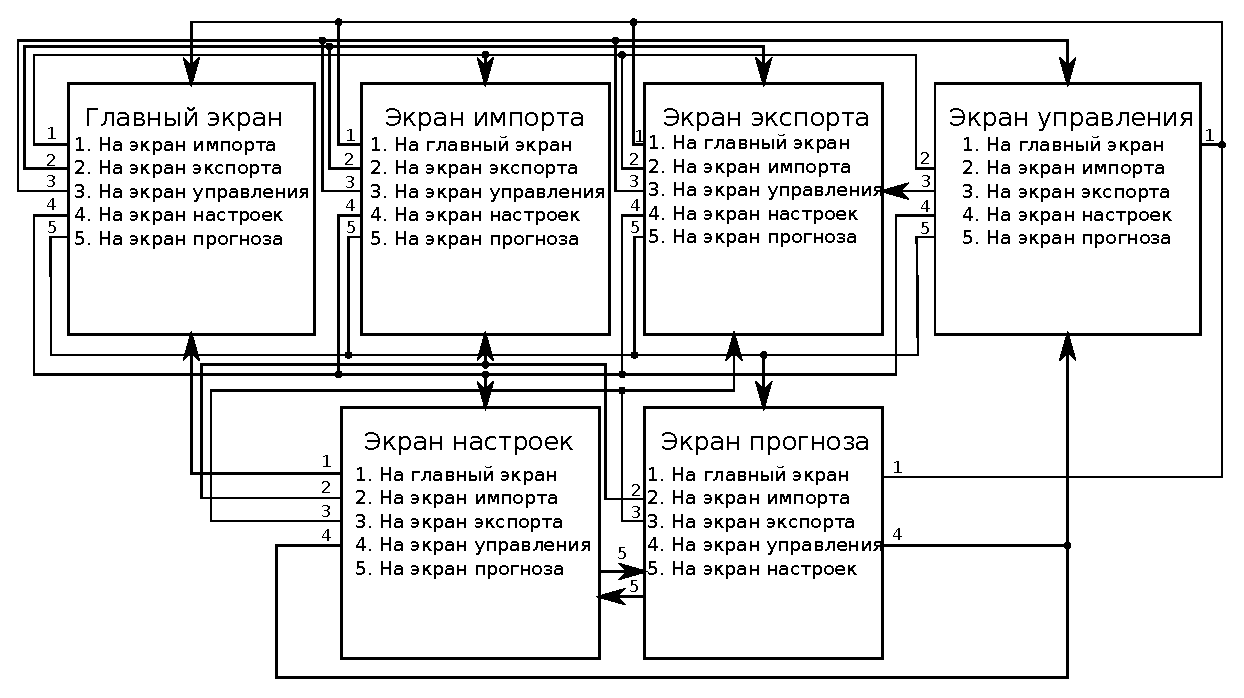
\includegraphics[angle=90,origin=c]{technology/dialog_generic}
%\caption{Обобщенный граф диалога взаимодействия с пользователем}
%\label{figure:dialog_generic}
%\end{figure}

\clearpage
\subsubsection{Разработка экранных форм}

При разработке экранных форму учитывались следующие требования к интерфейсу:
\begin{itemize}
\item Интерфейс должен быть удобен как для квалифицированного персонала, так и для новых пользователей АИС.
\item На каждом основном экране АИС должно присутствовать меню для перехода на другие экраны системы.
\item На каждом экране должны присутствовать только те элементы интерфейса, что необходимы для решения задачи, для которой экран предназначен.
\item Ввод данных должен быть интерактивным, то есть проводить проверку корректности вводимой информации и отображать причину ошибки в случае неправильно сформированных данных.
\end{itemize}

Основные экранные формы представлены в графической части проекта.

\clearpage
\subsection{Описание экранных форм}

\subsubsection{Главный экран}

  \begin{figure}[h!]
  \centering
  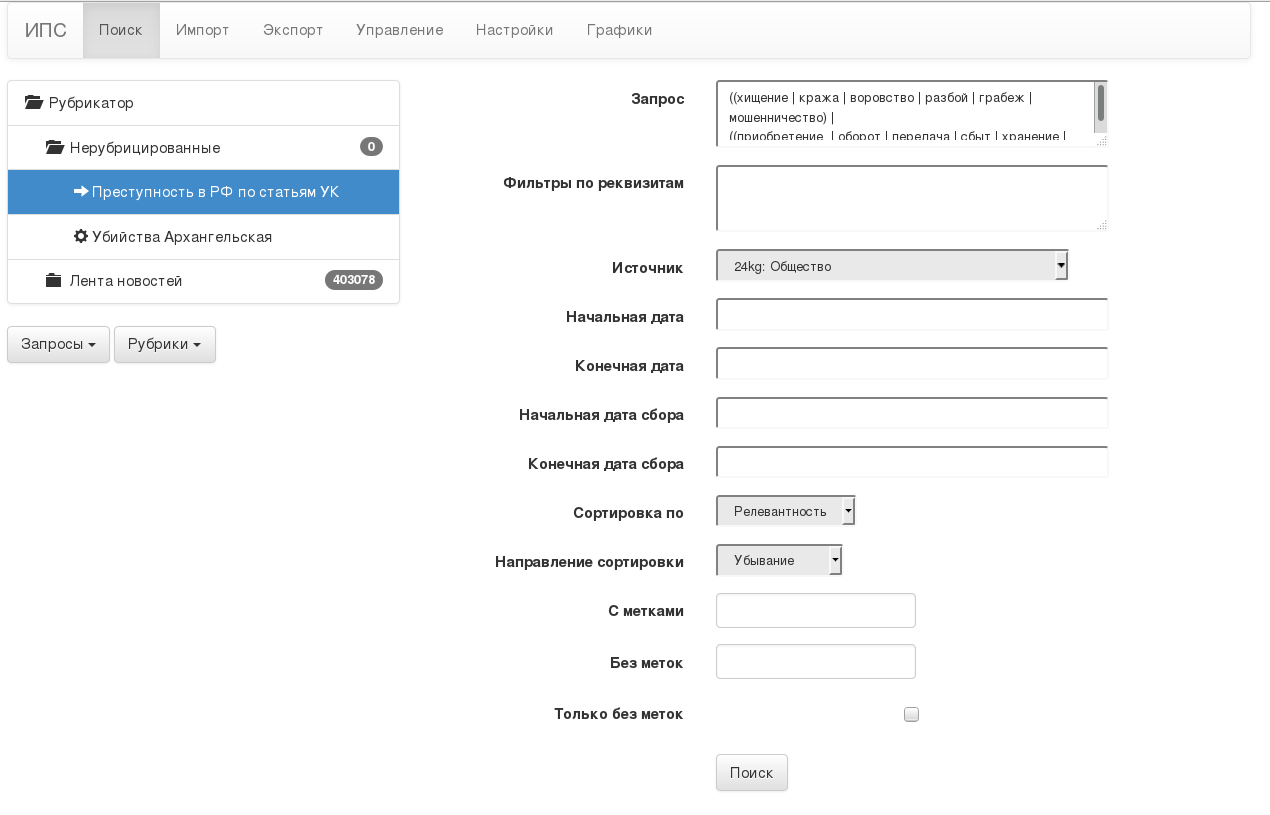
\includegraphics[width=0.9\linewidth]{technology/gui_main}
  \caption{Главный экран АИС}
  \label{figure:guiMain}
  \end{figure}

  На рис.~\ref{figure:guiMain} представлен вид главного экрана АИС. Экран содержит:
  \begin{itemize}
  \item Меню в верхней части экрана, через которое можно попасть на другие экраны системы.
  \item Рубрикатор в левой части экрана. Через рубрикатор пользователь может выбирать текущие категории документов, выбирать сохранённые запросы. Выпадающие панели под рубрикатором содержат действия над рубриками (создание, обновление, удаление, перемещение, экспорт из рубрики) и над сохранёнными запросами (создание, обновление, удаление). Рядом с названиями рубрик отображается количество документов в рубрике.
  \item Форма ввода запроса в правой части экрана. В форме присуствуют следующие поля:
  \begin{enumerate}
  \item Запрос -- тело формализованного запроса;
  \item Фильтры по реквизитам -- дополнительные ограничения на реквизиты документа;
  \item Источник -- выпадающий список из всех доступных источников документов;
  \item Начальная дата -- фильтрация по дате публикации документа. Задает начальное значение интервала;
  \item Конечная дата -- фильтрация по дате публикации документа. Задает конечное значение интервала;
  \item Начальная дата сбора -- фильтрация по дате сбора документа. Задает начальное значение интервала;
  \item Конечная дата сбора -- фильтрация по дате сбора документа. Задает конечное значение интервала;
  \item Сортировка по -- указание реквизита документа, по которому будет проводиться сортировка;
  \item Направление сортировки -- указание направления сортировки, по убыванию или по возрастанию;
  \item С метками -- перечисление меток документа, которые должны у него присутствовать;
  \item Без меток -- перечисление меток документа, которые должны у него отсутствовать;
  \item Только без меток -- специальный признак, при активации которого поиск будет проводиться только по документам, у которых нет никаких меток;
  \end{enumerate}

  \end{itemize}

  \begin{figure}[h!]
  \centering
  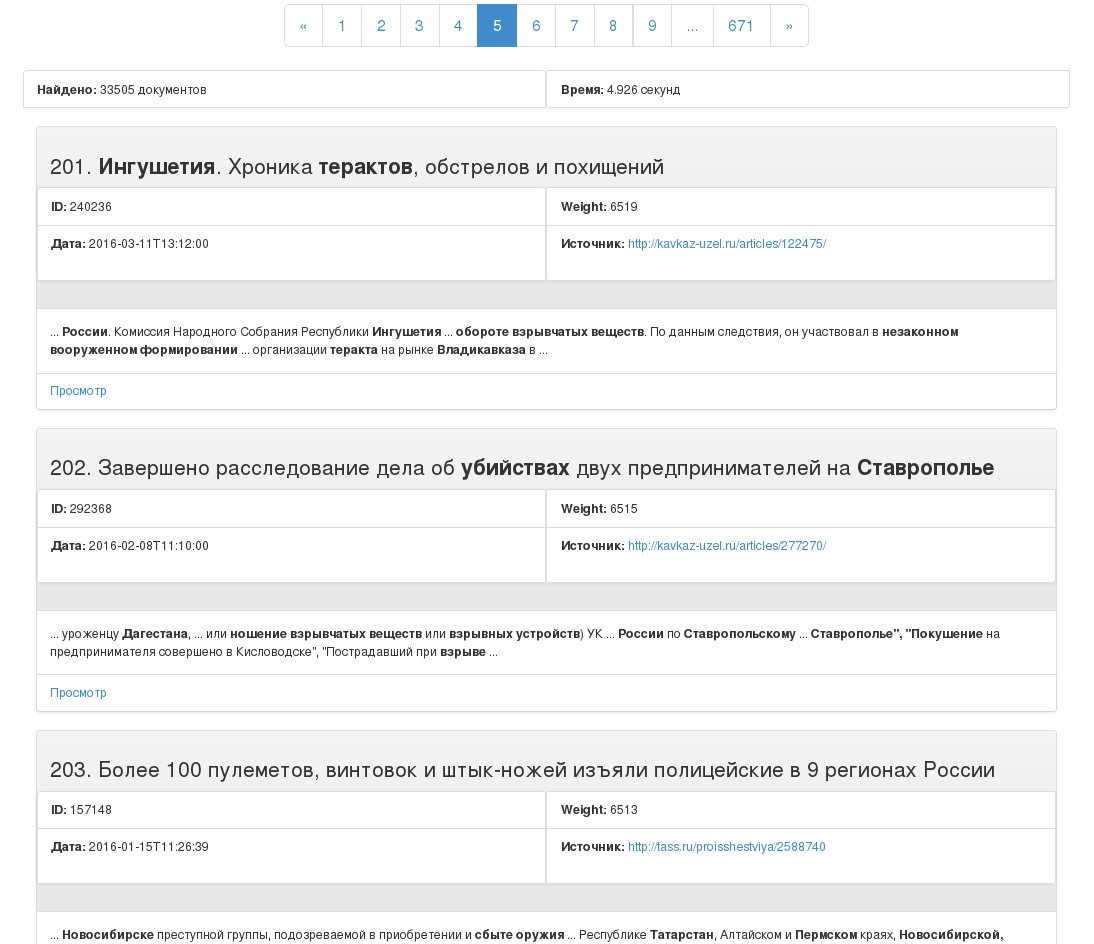
\includegraphics[width=0.9\linewidth]{technology/gui_main_results}
  \caption{Главный экран АИС, поисковая выдача}
  \label{figure:guiMainResults}
  \end{figure}

  После нажатия на кнопку <<Поиск>> в нижней части экрана пользователю отображается вторая часть данного экрана с поисковой выдачей (рис.~\ref{figure:guiMainResults}). Поисковая выдача может содержать множество документов, поэтому экран содержит кнопки перехода по страницам. Каждый элемент выдачи содержит название документа, его основные реквизиты и кусок текста, который подходит под заданный формализованный запрос. 

  \begin{figure}[h!]
  \centering
  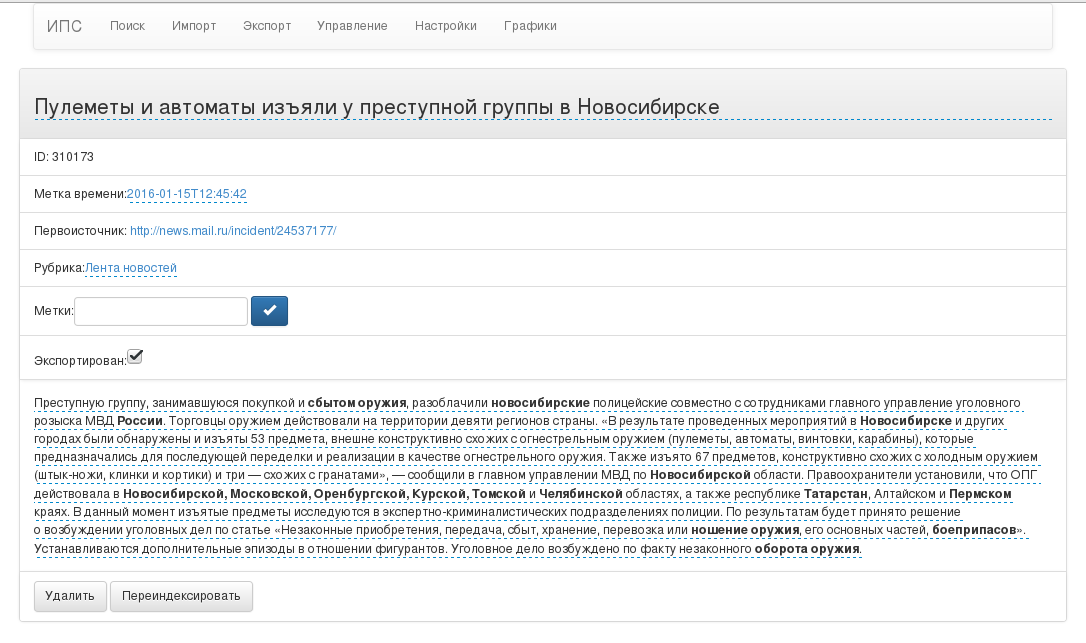
\includegraphics[width=0.9\linewidth]{technology/gui_main_document}
  \caption{Просмотр полного документа}
  \label{figure:guiMainDocument}
  \end{figure}

  Документ в элементе поисковой выдачи можно просмотреть отдельно с помощью ссылки <<Просмотр>> в нижней части элемента выдачи. Вид страницы документа представлен на рис.~\ref{figure:guiMainDocument}. Подробный вид документа содержит значения всех реквизитов, а также предоставляет возможность удаления или переиндексирования документа. Каждый реквизит, кроме идентификатора и источника, можно отредактировать путем щелчка мышкой на данных реквизита и ввода новых во всплывающем элементе ввода. Текст документа подсвечен согласно последнему выполненному запросу.

\clearpage
\subsubsection{Экран импорта}

  \begin{figure}[h!]
  \centering
  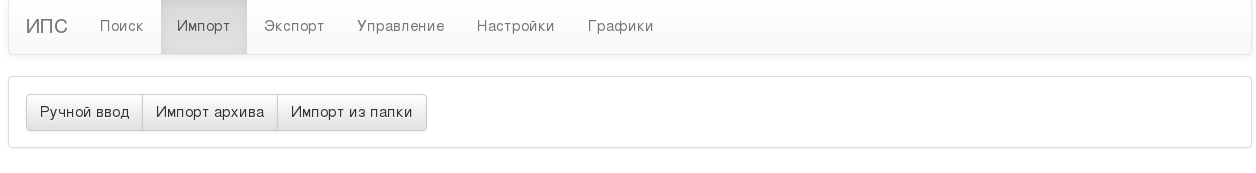
\includegraphics[width=0.9\linewidth]{technology/gui_import}
  \caption{Экран импорта документов}
  \label{figure:guiImport}
  \end{figure}

  На рис.~\ref{figure:guiImport} представлен вид экрана импорта документов. Экран содержит:
  \begin{itemize}
  \item Меню в верхней части экрана, через которое можно попасть на другие экраны системы.
  \item Кнопку перехода в ручной режим -- ввод документов через форму ввода поштучно, представлено на рис.~\ref{figure:guiImportSingle}.
  \item Кнопку перехода в режим архива -- отправка архива с несколькими документами. Интерфейс этого режима предназначен для загрузки очень объемных архивов с отображением процесса загрузки. Режим представлен на рис.~\ref{figure:guiImportArchive}.
  \item Кнопку запуска импорта из папки импорта -- при нажатии на эту кнопку происходит ручное инициирование сканирования папки импорта на новые документы.
  \end{itemize}

  \begin{figure}[h!]
  \centering
  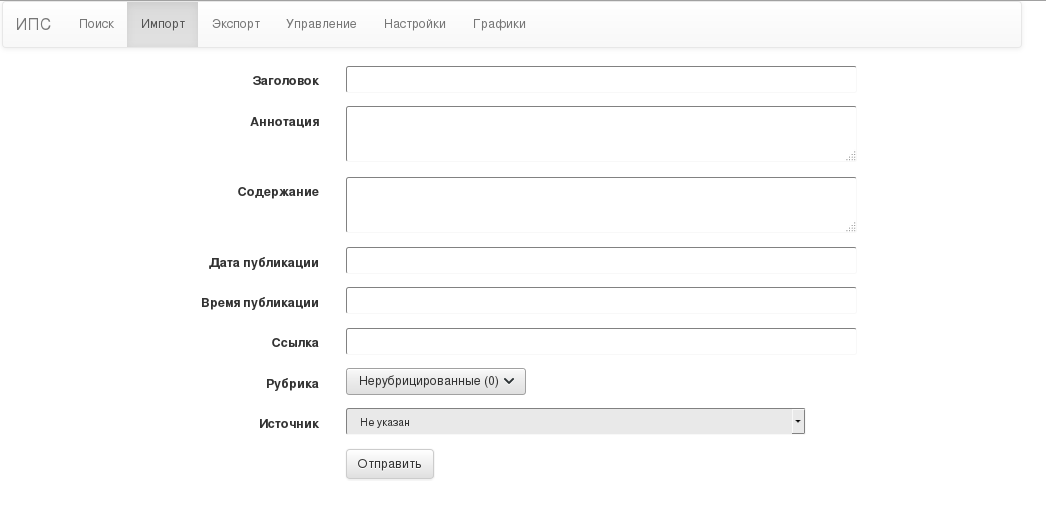
\includegraphics[width=0.9\linewidth]{technology/gui_import_single}
  \caption{Экран импорта документов, ручной режим}
  \label{figure:guiImportSingle}
  \end{figure}

  \begin{figure}[h!]
  \centering
  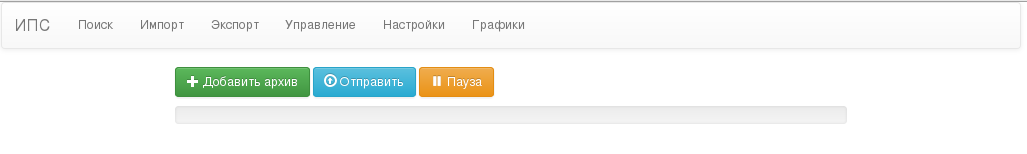
\includegraphics[width=0.9\linewidth]{technology/gui_import_archive}
  \caption{Экран импорта документов, режим архива}
  \label{figure:guiImportArchive}
  \end{figure}

\clearpage
\subsubsection{Экран экспорта}

  \begin{figure}[h!]
  \centering
  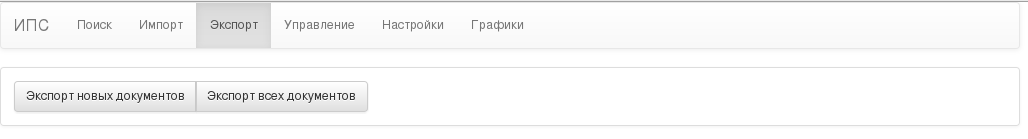
\includegraphics[width=0.9\linewidth]{technology/gui_export}
  \caption{Экран экспорта документов}
  \label{figure:guiExport}
  \end{figure}

  На рис.~\ref{figure:guiExport} представлен вид экрана экспорта документов. Экран содержит:
  \begin{itemize}
  \item Меню в верхней части экрана, через которое можно попасть на другие экраны системы.
  \item Кнопка запуска полного экспорта, при нажатии на которую начинается полный экспорт документов.
  \item Кнопка запуска инкрементального экспорта, при нажатии на которую начнется экспорт только еще не экспортированных документов.
  \end{itemize}

  При нажатии на любую из кнопок стартует операция система, список которых можно посмотреть на экране управления. Также во время экспорта на всех экранах системы отображается информационный элемент (рис.~\ref{figure:guiExportInfo}), а после завершения экспорта на экране экспорта отображается список готовых архивов, которые пользователь может скачать и перенести на другую развернутую АИС <<Волхв>>.

  \begin{figure}[h!]
  \centering
  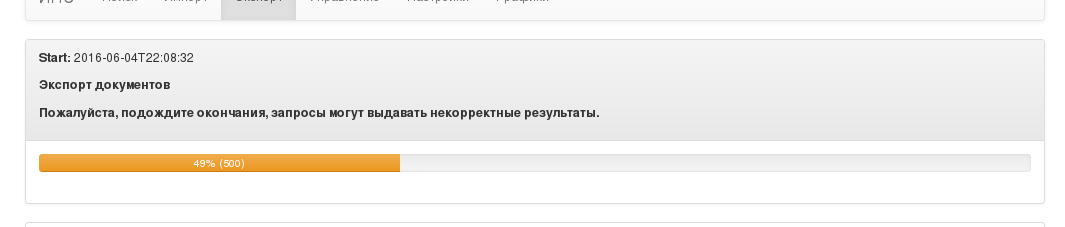
\includegraphics[width=0.9\linewidth]{technology/gui_export_info}
  \caption{Информационный элемент, который показывается на всех экранах АИС во время операции экспорта.}
  \label{figure:guiExportInfo}
  \end{figure}

\clearpage
\subsubsection{Экран управления}

  \begin{figure}[h!]
  \centering
  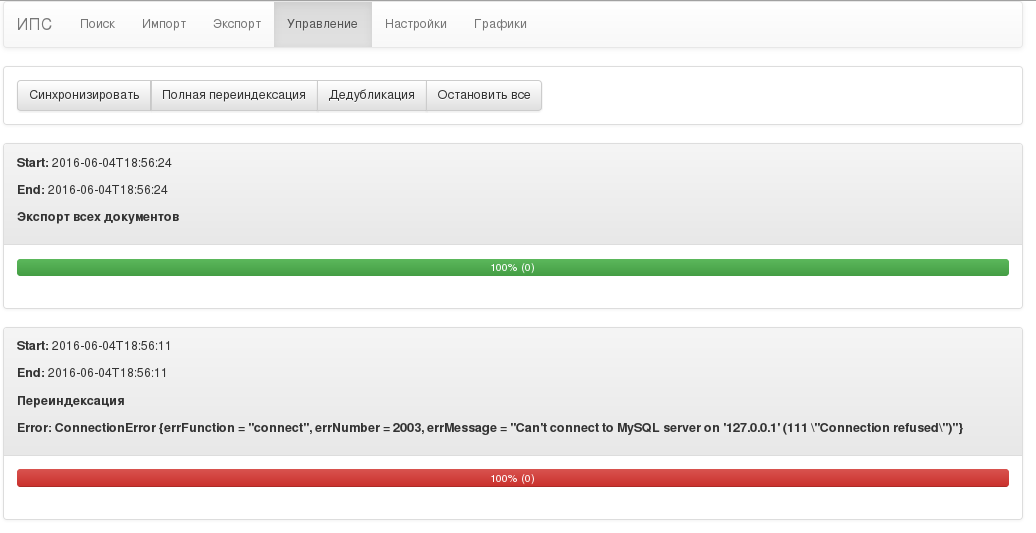
\includegraphics[width=0.9\linewidth]{technology/gui_resync}
  \caption{Экран управления операциями АИС}
  \label{figure:guiResync}
  \end{figure}

  На рис.~\ref{figure:guiResync} представлен вид экрана управления операциями АИС. Экран содержит:
  \begin{itemize}
  \item Меню в верхней части экрана, через которое можно попасть на другие экраны системы.
  \item Панель управления с кнопками запуска операций над базой документов: 
    \begin{enumerate}
      \item Синхронизировать -- запуск операции синхронизации индекса с базой документов, данная операция необходима при неполадках в системе для восстановления целостности индекса.
      \item Полная переиндексация -- запуск операции переиндексации базы документов, в отличии от синхронизации переиндексация удаляет весь индекс и перестраивает его с нуля. Данная операция нужна, когда меняются настройки индекса и для корректной его работы необходимо провести перестройку индекса.
      \item Дедубликация -- запуск операции удаления дублей из базы данных документов. При неаккуратном обращении с системой возможна ситуация, когда в базу были загружены дубли документов, данная операция находит и удаляет такие дубли.
      \item Остановить все -- прекращает выполнение всех операций, запущенных в данный момент.
    \end{enumerate}
  \item Список операций, запущенных или уже завершившихся. Для каждой операции отображается дата начала и конца работы. При аварийном завершении отображается текст ошибки и панель прогресса подсвечивается красным. При успешном завершении панель прогресса отображается зеленым цветом, а операции в процессе выполнения обозначаются желтым цветом.
  \end{itemize}

\clearpage
\subsubsection{Экран настроек}

\begin{figure}[h!]
\centering
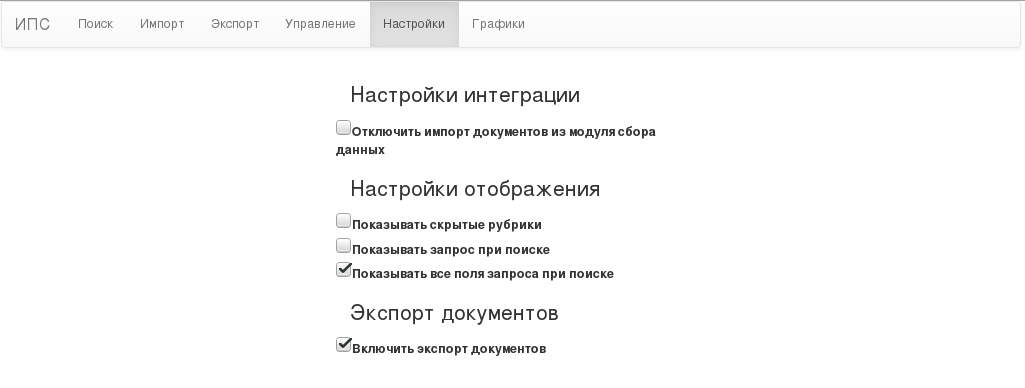
\includegraphics[width=0.9\linewidth]{technology/gui_options}
\caption{Экран настроек АИС}
\label{figure:guiOptions}
\end{figure}

На рис.~\ref{figure:guiOptions} представлен вид экрана настроек АИС. Экран содержит:
\begin{itemize}
\item Меню в верхней части экрана, через которое можно попасть на другие экраны системы.
\item Список настроек системы, каждая из которых представлена элементом <<checkbox>>:
\begin{enumerate}
  \item Отключение автоматического импорта документов из папки импорта. Необходимо при проведении технических работ над индексом, при которых нежелательно поступление новых документов в базу данных.
  \item Показ скрытых рубрик. Каждая рубрика может иметь признак скрытости и не отображаться пользователю через web-интерфейс. Такие рубрики используются для интеграции с другими системами и позволяют делать сохраненные формализованные запросы  и рубрики для использования другими сервисами.
  \item Показ запроса при поиске. При включенном признаке система будет показывать полученный поисковый запрос перед выборкой документов, пример такого запроса представлен на рис.~\ref{figure:guiOptionsQuery}.
  \item Показ всех полей при поиске. При отключенном признаке система не будет показывать редко используемые поля в форме ввода поискового запроса.
  \item Включить экспорт документов. При отключенном признаке система скроет все элементы, относящиеся к функциональности экспорта документов. Данная опция полезна для реплик АИС, для которых экспорт документов не используется, а только мешает пользователям.
\end{enumerate}
\end{itemize}

\begin{figure}[h!]
\centering
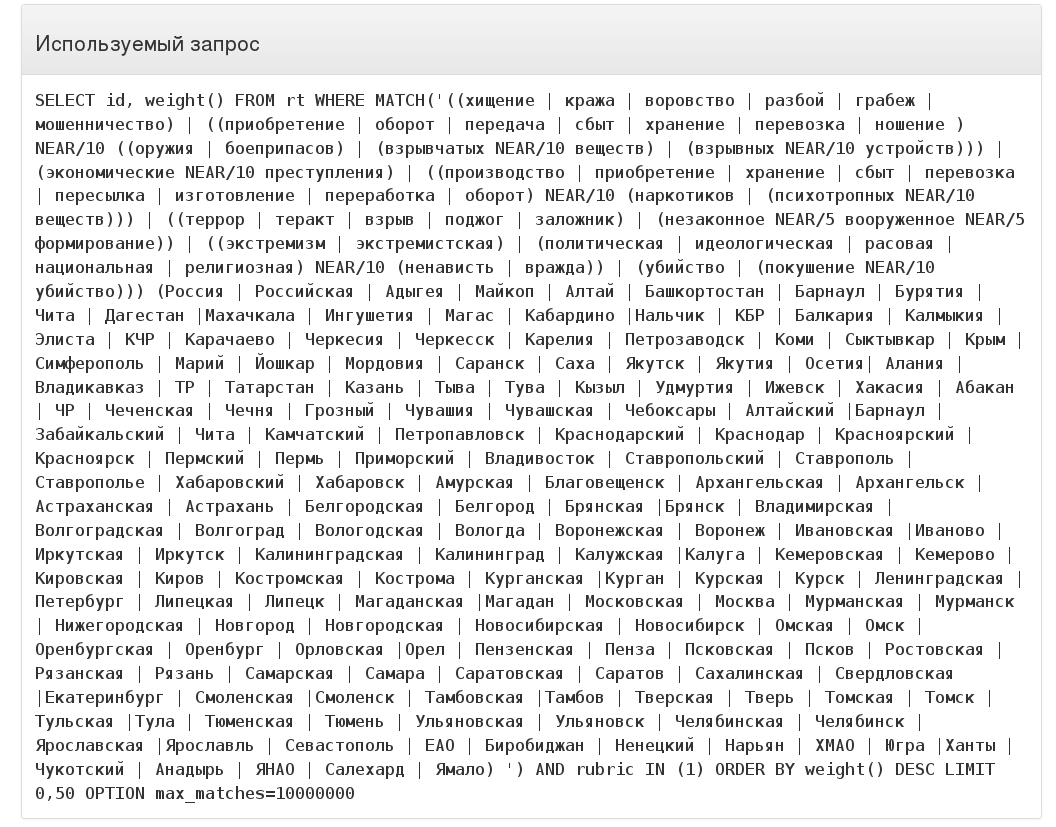
\includegraphics[width=0.9\linewidth]{technology/gui_options_query}
\caption{Элемент вывода запроса при поиске}
\label{figure:guiOptionsQuery}
\end{figure}


\clearpage
\subsubsection{Экран прогнозирования} 

\begin{figure}[h!]
\centering
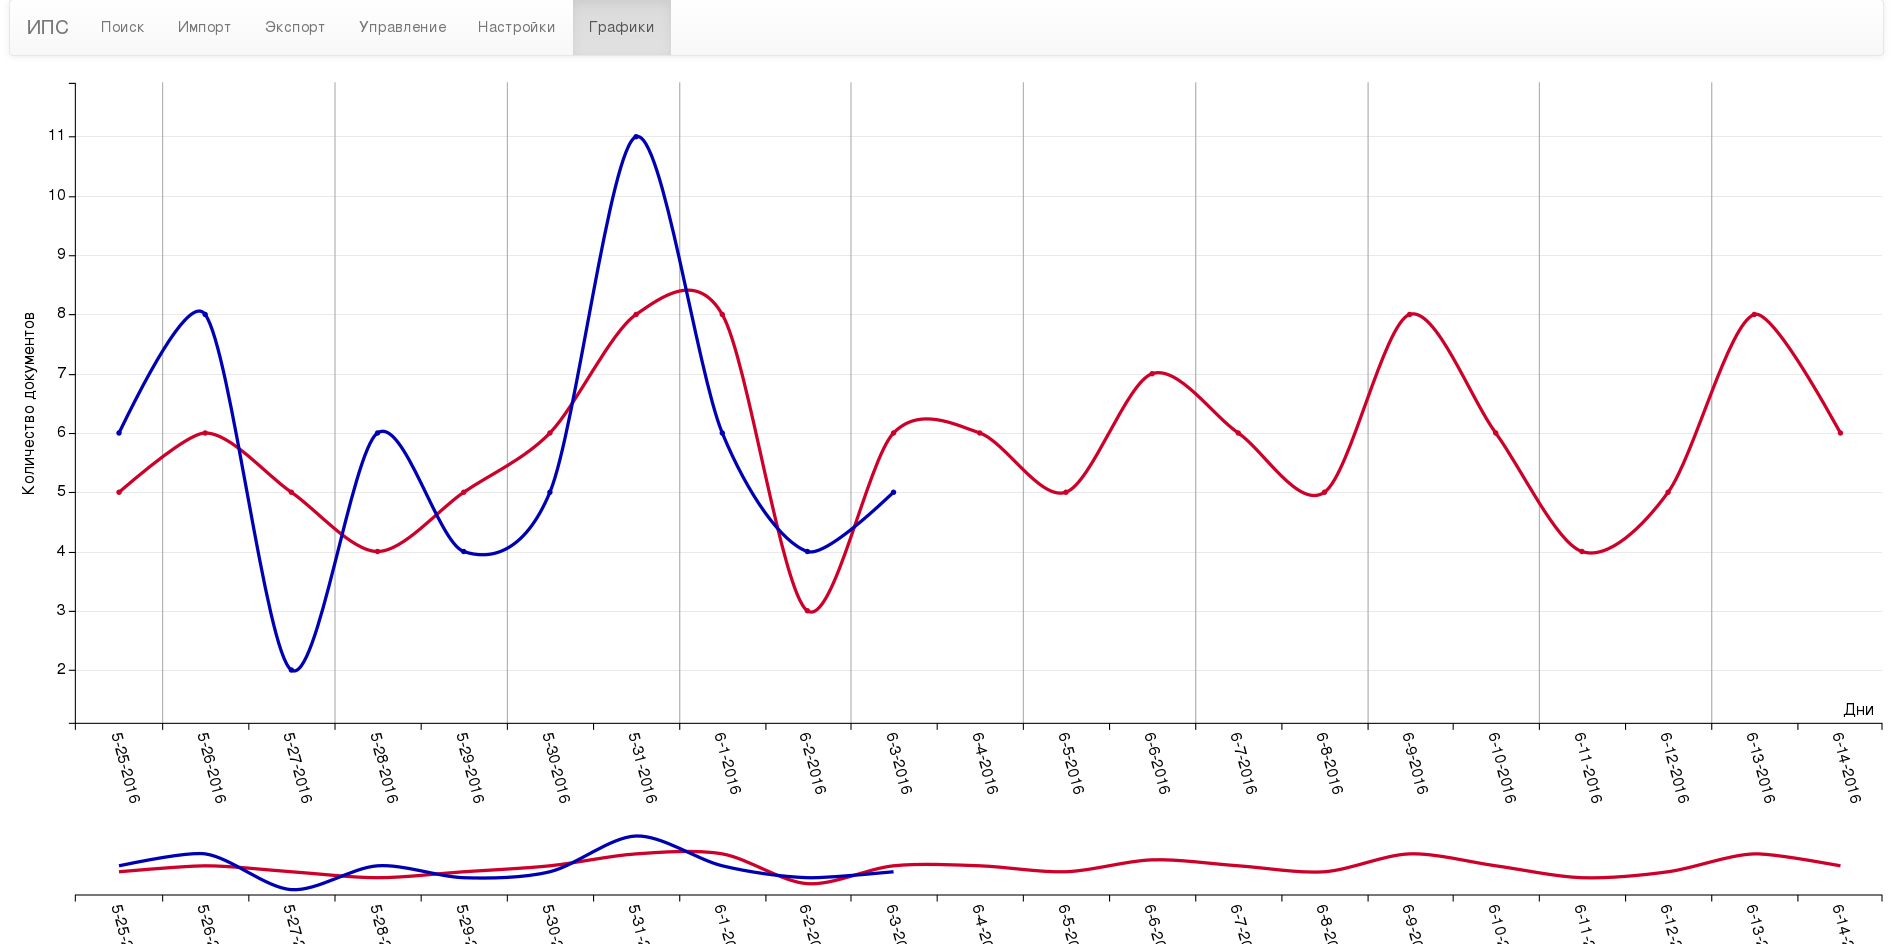
\includegraphics[width=0.9\linewidth]{technology/gui_predict1}
\caption{Экран прогнозирования АИС, часть 1}
\label{figure:guiPredict2}
\end{figure}

\begin{figure}[h!]
\centering
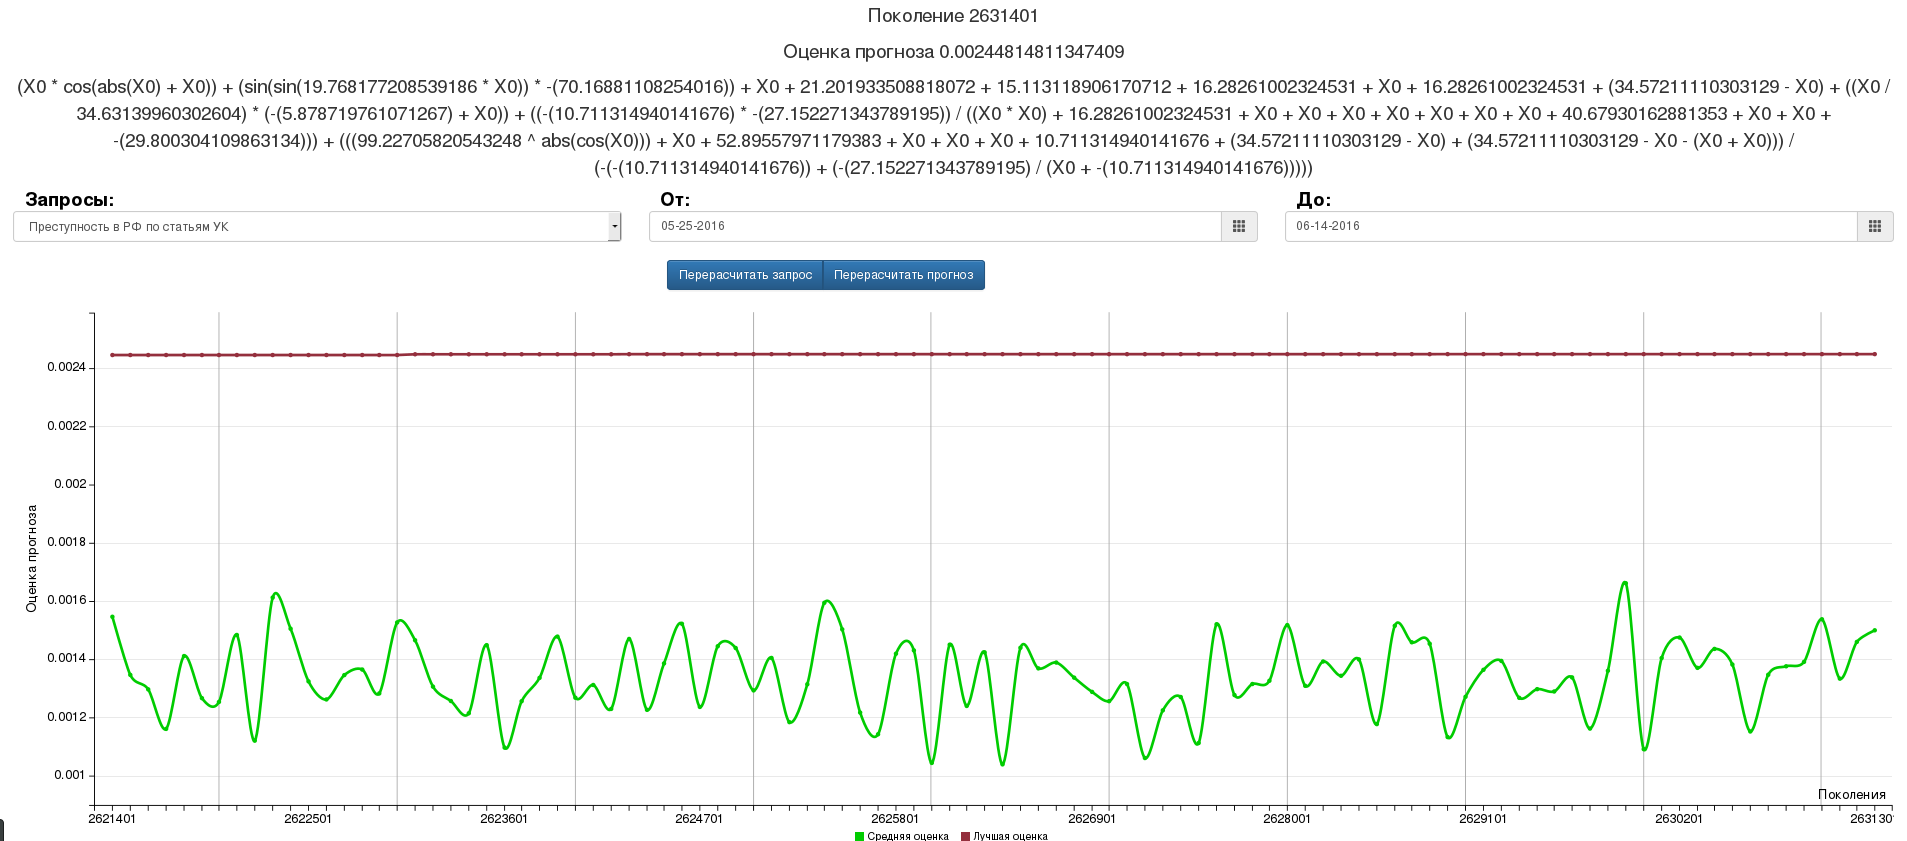
\includegraphics[width=0.9\linewidth]{technology/gui_predict2}
\caption{Экран прогнозирования АИС, часть 2}
\label{figure:guiPredict1}
\end{figure}

На рис.~\ref{figure:guiPredict1} и рис.~\ref{figure:guiPredict2} представлен вид экрана прогнозирования АИС. Экран содержит:
\begin{itemize}
\item Меню в верхней части экрана, через которое можно попасть на другие экраны системы.
\item Элемент графиков, который содержит два подграфика:
\begin{enumerate}
  \item Синий график -- значения количества документов, удовлетворяющих сохраненному запросу по дням. 
  \item Красный график -- график прогноза количества документов по дням, в том числе и ретроспективный прогноз для оценки качества прогнозирования.
\end{enumerate}
\item Миниатюра графиков -- отображение всего рассматриваемого периода времени. Пользователь может выбрать интервал внутри миниатюры, и верхний график подстроится для отображения под заданный интервал времени.
\item Число поколений прогноза -- отображает количество поколений, прошедших в эволюционном алгоритме, с начала прогнозирования.
\item Количественная оценка качества прогнозирования -- среднеквадратичное отклонение прогноза от реальных данных.
\item Аналитическая формула прогноза -- аналитическая функция, полученная в результате символьной регрессии на основе эволюционных алгоритмов.
\item Вспомогательный график для оценки качества прогноза:
\begin{enumerate}
\item Коричневая линия отображает лучшие значение функции приспособленности от поколения популяций. Данная функция должна монотонно не убывать при низменности реальных данных.
\item Зеленая линия отображает среднее значение функции приспособленности от поколения популяций. Данная функция должна быть ниже коричневой, что свидетельствует от генетическом разнообразии популяций.
\end{enumerate}
\end{itemize}


%===========================================================================
% Исследовательская часть
\section{Исследовательская часть}

%===========================================================================
% Организационно -- Экономическая часть
\include{orgecon/stages}
\include{orgecon/costs}
\include{orgecon/workers}
\include{orgecon/salary}
\include{orgecon/equip}
\include{orgecon/workplace}
\include{orgecon/overheads}
\include{orgecon/others}

%===========================================================================
% ОБЖ и Экология
\include{obzeco/analysis}
\include{obzeco/normalize}
\include{obzeco/expertise}
\include{obzeco/results}

%===========================================================================
\clearpage
\addcontentsline{toc}{chapter}{\bibname}
\bibliographystyle{utf8gost705u}  %% стилевой файл для оформления по ГОСТу
\bibliography{biblio}     %% имя библиографической базы (bib-файла) 

\end{document}